\documentclass[a4paper,12pt]{article}

% Pakete laden
\usepackage[utf8]{inputenc} % Zeichenkodierung
\usepackage[ngerman,english]{babel} % Sprache
\usepackage{microtype}      % Schriftbild und den Zeilenumbruch verbessern
\usepackage{graphicx}       % Grafiken
\usepackage{csquotes}       % Zitate
\usepackage[style=ieee]{biblatex} % Literaturverzeichnis
\usepackage{fancyhdr}       % Kopf- und Fußzeilen
\usepackage[T1]{fontenc}    % Schriftart
\usepackage{uarial}         % Arial
\usepackage{parskip}        % Abstand zwischen Absätzen
\usepackage[nopostdot,nonumberlist,acronym,automake,toc,section]{glossaries} % Abkürzungsverzeichnis
\usepackage{titlesec}       % Section- und Subsection-Überschriften
\usepackage[colorlinks=false,pdfborder={0 0 0}]{hyperref} % Hyperlink für Inhaltsverzeichnis und Quellen
\usepackage{nameref}
\usepackage[nottoc,notbib,section]{tocbibind}
\usepackage{url}            % bessere Darstellung von Links
\usepackage{enumitem}       % Aufzählungen
\usepackage{booktabs}       % Tabellen mit schöneren Linien
\usepackage{multirow}       % Tabellen mit mehreren Zeilen
\usepackage{longtable}      % Für mehrseitige Tabellen
\usepackage{makecell}       % Für Zellen in Tabellen
\usepackage{lipsum}         % Dummy Text
\usepackage{xcolor}
\usepackage{xparse}
\usepackage{amssymb}      % Mathematische Symbole wie \mathbb
\usepackage{needspace}
\usepackage{float}


% Ränder einstellen
\usepackage[
    left=2.5cm, 
    right=2.5cm, 
    top=0cm, 
    bottom=2.5cm,
    nomarginpar,
    includehead,
    headheight=2.5cm,
    headsep=1cm
]{geometry}


% Anpassung der Referenzformatierung
\NewDocumentCommand{\fautoref}{m}{\textbf{\autoref{#1}}}
\NewDocumentCommand{\fsecref}{m}{\textbf{\hyperref[#1]{\ref*{#1} \nameref*{#1}}}}
\NewDocumentCommand{\shortsecref}{m}{\textbf{\hyperref[#1]{\nameref*{#1}}}}

% Definiere Bibliografie-Treiber für @video
\DeclareBibliographyAlias{video}{online}
\DeclareBibliographyAlias{software}{online}

% Schriftart ändern
\renewcommand{\familydefault}{\sfdefault}
\usepackage{setspace}

% Setzt den Zeilenabstand
\onehalfspacing

% Setze den Abstand zwischen Absätzen
\setlength{\parskip}{0.75cm}

% Abstand vor und nach Section- und Subsection-Überschriften anpassen
\titlespacing{\section}{0pt}{1.5cm}{0.75cm}
\titlespacing{\subsection}{0pt}{1.25cm}{0.5cm}
\titlespacing{\subsubsection}{0pt}{0.75cm}{0.25cm}



% Paket und Style fuer Code-Listings
\usepackage{listings}
\usepackage{color}
\renewcommand{\lstlistingname}{Listing}

\definecolor{codebg}{RGB}{245,245,245}
\definecolor{codekeyword}{RGB}{0,0,150}
\definecolor{codecomment}{RGB}{100,100,100}
\definecolor{codestring}{RGB}{163,21,21}
\definecolor{codetorch}{RGB}{170,60,0}

% PyTorch/NumPy-Bezeichner, die im Quellcode der Kapitel als eigene
% Keyword-Klasse (Klassen, Module, Tensor-Methoden) hervorgehoben werden
\lstdefinestyle{bachelorarbeit}{
    backgroundcolor=\color{codebg},
    basicstyle=\ttfamily\small,
    keywordstyle=\color{codekeyword}\bfseries,
    keywordstyle=[2]\color{codetorch}\bfseries,
    commentstyle=\color{codecomment}\itshape,
    stringstyle=\color{codestring},
    numbers=left,
    numberstyle=\tiny\color{gray},
    numbersep=8pt,
    frame=single,
    breaklines=true,
    breakatwhitespace=false,
    showstringspaces=false,
    tabsize=4,
    captionpos=b,
    morekeywords=[2]{
        torch, nn, np,
        DataLoader, Dataset, GRURegressor,
        Adam, MSELoss,
        cuda, is_available, manual_seed, seed,
        no_grad, clip_grad_norm_, utils,
        state_dict, load_state_dict, parameters,
        zero_grad, backward, step, train, eval,
        to, from_numpy, tensor, detach, cpu, clone,
        float32
    },
    literate=
        {ä}{{\"a}}1 {ö}{{\"o}}1 {ü}{{\"u}}1
        {Ä}{{\"A}}1 {Ö}{{\"O}}1 {Ü}{{\"U}}1
        {ß}{{\ss}}1,
}

\lstset{style=bachelorarbeit}


% Bilder Verzeichnis einbinden
\graphicspath{{images/}}
% Literaturdatei einbinden
\addbibresource{literature.bib}

% Kopfzeile definieren
\pagestyle{fancy}
\fancyhead{} % Leert Kopf- und Fußzeile
\renewcommand{\headrulewidth}{0pt}
\fancyhead[c]{
    
\includegraphics[width=3.5cm]{hitachi} \hfill
    
\includegraphics[width=3.5cm]{dhbw}
}

% Fußzeile definieren
\cfoot{\textbf{\thepage}}
\pagenumbering{roman}

% Akronyme
\makeglossaries
\newcommand{\acrlongshort}[1]{\glsentrylong{#1} (\glsentryshort{#1})}
\newacronym{ATO}{ATO}{Automatic Train Operation}
\newacronym{RL}{RL}{Reinforcement Learning}
\newacronym{DRL}{DRL}{Deep Reinforcement Learning}
\newacronym{EDA}{EDA}{Exploratory Data Analysis}
\newacronym{MSE}{MSE}{Mean Squared Error}
\newacronym{SL}{SL}{Supervised Learning}
\newacronym{BC}{BC}{Behavior Cloning}
\newacronym{LR}{LR}{Learning Rate}
\newacronym{Adam}{Adam}{Adaptive Moment Estimation}
\newacronym{AdamW}{AdamW}{Adam with Weight Decay}
\newacronym{Adagrad}{Adagrad}{Adaptive Gradient Algorithm}
\newacronym{SGD}{SGD}{Stochastic Gradient Descent}
\newacronym{RMSprop}{RMSprop}{Root Mean Square Propagation}
\newacronym{IL}{IL}{Imitation Learning}
\newacronym{MLP}{MLP}{Multi-Layer Perceptron}
\newacronym{RNN}{RNN}{Recurrent Neural Network}
\newacronym{LSTM}{LSTM}{Long Short-Term Memory}
\newacronym{GRU}{GRU}{Gated Recurrent Unit}
\newacronym{ERM}{ERM}{Empirical Risk Minimization}
\newacronym{PPO}{PPO}{Proximal Policy Optimization}
\newacronym{SAC}{SAC}{Soft Actor-Critic}
\newacronym{DDQN}{DDQN}{Double Deep Q-Network}
\newacronym{DAgger}{DAgger}{Dataset Aggregation}
\newacronym{PID}{PID}{Proportional-Integral-Derivative}
\newacronym{PI}{PI}{Proportional-Integral}
\newacronym{NaN}{NaN}{Not a Number}
\newacronym{KI}{KI}{Künstliche Intelligenz}
\newacronym{ML}{ML}{Machine Learning}
\newacronym{MAE}{MAE}{Mean Absolute Error}
\newacronym{RMSE}{RMSE}{Root Mean Squared Error}
\newacronym{WSRL}{WSRL}{Warm-Start Reinforcement Learning}
\newacronym{ALVINN}{ALVINN}{Autonomous Land Vehicle In a Neural Network}
\newacronym{FE}{FE}{Feature Engineering}
\newacronym{BPTT}{BPTT}{Backpropagation Through Time}
\newacronym{ODD}{ODD}{Operational Design Domain}
\newacronym{MI}{MI}{Mutual Information}
\newacronym{OLS}{OLS}{Ordinary Least Squares}
\newacronym{LZB}{LZB}{Linienzugbeeinflussung}
\newacronym{IID}{IID}{Independent and Identically Distributed}
\newacronym{CCS}{CCS}{Control Command and Signalling}
\newacronym{ETCS}{ETCS}{European Train Control System}
\newacronym{RST}{RST}{Rolling Stock}
\newacronym{ORD}{ORD}{On-board Recording Device}
\newacronym{GPS}{GPS}{Global Positioning System}
\newacronym{MDP}{MDP}{Markov Decision Process}
\newacronym{POMDP}{POMDP}{Partially Observable Markov Decision Process}
\newacronym{SI}{SI}{Internationales Einheitensystem}
\newacronym{DL}{DL}{Deep Learning}
\newacronym{EMA}{EMA}{Exponential Moving Average}
\newacronym{AMP}{AMP}{Automatic Mixed Precision}
\newacronym{GPU}{GPU}{Graphics Processing Unit}
\newacronym{CPU}{CPU}{Central Processing Unit}
\newacronym{TPU}{TPU}{Tensor Processing Unit}

% ---------------------------------------------------------------------------
% Abkürzungs-Anzeige mit Auffrischung pro Section
%   - Allererste Verwendung im Dokument:  Langform (Kurzform)
%   - Erste Verwendung in einer neuen Section (bereits zuvor verwendet):
%                                          Kurzform (Langform)
%   - Weitere Verwendungen in derselben Section: nur Kurzform
% Die Auffrischung erfolgt nur bei \section, nicht bei \subsection/\subsubsection.
% ---------------------------------------------------------------------------

% Kurzform mit korrektem Plural und Groß-/Kleinschreibung
\newcommand{\glsAbbrShort}{%
  \glsifplural
    {\glscapscase{\glsentryshortpl{\glslabel}}{\Glsentryshortpl{\glslabel}}{\glsentryshortpl{\glslabel}}}%
    {\glscapscase{\glsentryshort{\glslabel}}{\Glsentryshort{\glslabel}}{\glsentryshort{\glslabel}}}%
}
% Langform mit korrektem Plural und Groß-/Kleinschreibung
\newcommand{\glsAbbrLong}{%
  \glsifplural
    {\glscapscase{\glsentrylongpl{\glslabel}}{\Glsentrylongpl{\glslabel}}{\glsentrylongpl{\glslabel}}}%
    {\glscapscase{\glsentrylong{\glslabel}}{\Glsentrylong{\glslabel}}{\glsentrylong{\glslabel}}}%
}

\defglsentryfmt{%
  \ifglsused{\glslabel}%
    {% bereits in dieser Section verwendet -> nur Kurzform
      \glsAbbrShort\glsinsert
    }%
    {% erste Verwendung in dieser Section
      \ifcsdef{glsever@\glslabel}%
        {% schon einmal (in einer fruheren Section) verwendet -> Kurzform (Langform)
          \glsAbbrShort\glsinsert\ (\glsAbbrLong)%
        }%
        {% allererste Verwendung im gesamten Dokument -> Langform (Kurzform)
          \glsAbbrLong\glsinsert\ (\glsAbbrShort)%
          \csgdef{glsever@\glslabel}{1}%
        }%
    }%
}

% Bei jeder neuen \section den "in dieser Section verwendet"-Status zuruecksetzen
\AtBeginDocument{%
  \pretocmd{\section}{\glsresetall}{}{%
    \PackageWarning{acronyms}{Konnte \string\section\space nicht patchen}%
  }%
}


% Definitionen
\newcommand{\projName}{Neuronale Modellierung realer Fahrstrategien im Schienenverkehr auf Basis historischer Betriebsdaten}

\begin{document}
    \selectlanguage{ngerman}

    % Titelseite
    \begin{titlepage}
    \thispagestyle{fancy}
    \fancyfoot{}
    \centering

    \vspace*{0cm}
    {\Huge\bfseries Bachelorarbeit \\ \Large \projName\par}
    \vspace{1.5cm}
    {\Large Anton Engels\par}
    \vspace{1.0cm}
    {\large Embedded Systems-General Engineering\par}
    \vspace{0.5cm}
    {\large Duale Hochschule Baden-Württemberg Stuttgart\par}
    \vspace{2.0cm}
    {\large \today\par}

    \vfill
    \begin{tabular}{l l}
        Bearbeitungszeitraum: & 15.6.2026 - 30.09.2026 \\
        \vspace{0.25cm}
        Matrikelnummer, Kurs: & 8910366, TES23 \\
        \vspace{0.25cm}
        Ausbildungsfirma: & Hitachi Rail GTS Deutschland GmbH \\
        Betreuer der Ausbildungsfirma: & Wolfgang Reza Sharavi \& Joel Mwaka \\
    \end{tabular}
    \vspace{2cm}

\end{titlepage}

    \newpage
    \setcounter{page}{2}

    % Erklärung
    \vspace*{2cm}
{\setlength{\fboxsep}{0.5cm}\fbox{\parbox{0.94\columnwidth}{
\begin{center}
\textbf{Sperrvermerk}
\end{center}
\vspace{0.5cm}

Die vorliegende Bachelorarbeit beinhaltet interne vertrauliche Informationen der Hitachi Rail GTS Deutschland GmbH. 
Die Weitergabe des Inhaltes der Arbeit und eventuell beiliegender Zeichnungen und Daten im Gesamten oder in Teilen ist
grundsätzlich untersagt. Es dürfen keinerlei Kopien oder Abschriften - auch in digitaler Form - gefertigt werden. 
Ausnahmen bedürfen der schriftlichen Genehmigung der Hitachi Rail GTS Deutschland GmbH.\\
Die Bachelorarbeit ist nur den Hochschulbetreuern zugänglich zu machen.
}}}
\vspace*{2cm}

\begin{center}
\textbf{Erklärung}
\end{center}

Ich versichere hiermit, dass ich die vorliegende Bachelorarbeit mit dem Thema „\projName“ 
selbstständig verfasst und keine anderen als die angegebenen Quellen und Hilfsmittel benutzt habe.
Eine Übersicht der dabei verwendeten Hilfsmittel ist im Anhang dargestellt.

Ich versichere zudem, dass die eingereichte elektronische Fassung mit der gedruckten Fassung übereinstimmt.

\vspace{3cm}
% Unterschriftfeld
\noindent
\begin{tabular}{l r}
    \textbf{71254 Ditzingen, \today} &
    \hspace{1cm} \underline{\hspace{6cm}}
\end{tabular}

    \newpage

    % Zusammenfassung
    \begin{abstract}
Der Einsatz von Reinforcement Learning zur automatisierten Zugsteuerung scheitert in der Praxis häufig an fehlender geeigneter Initialisierung: Agenten ohne fachliche Vorprägung konvergieren schlecht, während eine rein simulative Offline-Initialisierung dazu führt, dass Modelle Trainingsstrecken auswendig lernen statt eine generalisierbare Strategie zu erlernen. Diese Arbeit untersucht daher, ob sich aus historischen Betriebsdaten per Behavior Cloning ein neuronales Netz trainieren lässt, das eine generalisierbare Fahrstrategie erlernt und als Ausgangspunkt für zukünftige Reinforcement-Learning-Anwendungen dienen kann. Auf Basis realer Sensordaten einer Güterverkehrsstrecke werden eine deterministische Preprocessing-Pipeline und eine fahrtenbasierte Datenaufteilung zur Vermeidung von Data Leakage entwickelt. In einem dreistufigen Auswahlprozess wird ein LSTM-Netz (128-64-256-128, 650.369 Parameter) mit Adam-Optimierer und Smooth-L1-Verlust bestimmt und trainiert. Die Evaluation zeigt, dass das Modell eine Persistenz-Baseline bei regressionsbasierten Kennzahlen deutlich übertrifft, bei seltenen, dynamischen Manövern jedoch schwächelt, vermutlich aufgrund der begrenzten Datenbasis von rund 178 Stunden. Die Arbeit erbringt damit einen Machbarkeitsnachweis, zeigt aber zugleich, dass eine robuste Fahrstrategie eine deutlich umfangreichere Datengrundlage voraussetzt.
\end{abstract}
\selectlanguage{english}
\begin{abstract}
Applying reinforcement learning to automated train control is often hampered by the lack of suitable initialization: agents without prior domain knowledge tend to converge poorly, while purely simulation-based offline initialization risks models memorizing training routes instead of learning a generalizable strategy. This thesis therefore investigates whether a neural network can be trained on historical operational data via behavior cloning to learn a generalizable train driving strategy that can serve as a starting point for future reinforcement learning applications. Based on real sensor data from a freight rail line, a deterministic preprocessing pipeline and a trip-based data split to prevent data leakage are developed. Through a three-stage selection process, an LSTM network (128-64-256-128, 650,369 parameters) with the Adam optimizer and a Smooth-L1 loss function is determined and trained. Evaluation shows that the model clearly outperforms a persistence baseline on regression-based metrics but struggles with rare, dynamic maneuvers, likely due to the limited data basis of roughly 178 hours. The thesis thus provides a proof of concept, while also showing that a robust driving strategy requires a substantially larger data foundation.
\end{abstract}
\selectlanguage{ngerman}
    \newpage

    % Inhaltsverzeichnis
    \tableofcontents


    % Abbildungsverzeichnis
    \phantomsection
    \listoffigures
    \newpage
    
    % Tabellenverzeichnis
    \phantomsection
    \listoftables
    \newpage

    % Abkürzungsverzeichnis
    \begingroup
    \setstretch{.5}
    \glsaddall
    \printglossary[type=\acronymtype,title=Abkürzungsverzeichnis]
    \newpage
    \renewcommand{\glsgroupskip}{}
    \endgroup
    
    \newpage

    % Formelgr\"o\ss en und Einheiten
    \phantomsection
\section*{Formelgr\"o\ss en und Einheiten}
\addcontentsline{toc}{section}{Formelgr\"o\ss en und Einheiten}

\begingroup
\renewcommand{\arraystretch}{1.5}
\begin{longtable}{@{} >{\raggedright\arraybackslash}p{4.0cm} >{\raggedright\arraybackslash}p{2.5cm} >{\raggedright\arraybackslash}p{9.5cm} @{}}
        \textbf{Kurzzeichen} & \textbf{Einheit} & \textbf{Benennung} \\ \hline
        \endfirsthead
        \textbf{Kurzzeichen} & \textbf{Einheit} & \textbf{Benennung} \\ \hline
        \endhead
        $A_{\mathrm{Richt}}$ & \% & Richtungs-Accuracy \\
        $A_{\mathrm{Tol}}$ & \% & Toleranz-Accuracy \\
        $a_t$ & - & Aktion zum Zeitpunkt $t$ (normiert) \\
        $C_t$ & - & Zellzustand des LSTM zum Zeitpunkt $t$ \\
        $\mathcal{D}$ & - & Datensatz \\
        $d$ & - & Anzahl der Eingangsmerkmale \\
        $f_\theta$ & - & Modellfunktion \\
        $h_t$ & - & Hidden State zum Zeitpunkt $t$ \\
        $I$ & - & Einheitsmatrix \\
        $\mathcal{L}(\theta)$ & - & Verlustfunktion \\
        $\mathcal{L}_{\mathrm{MSE}}(\theta)$ & - & Mittlerer quadratischer Verlust \\
        $\mathcal{L}_{\mathrm{total}}(\theta)$ & - & Gesamter Verlust einschlie\ss lich Regularisierung \\
        $N$ & - & Anzahl der Datenpunkte beziehungsweise Fenster \\
        $o_t$ & - & Beobachtung zum Zeitpunkt $t$ \\
        $P_{\mathrm{deploy}}(X)$ & - & Eingabeverteilung w\"ahrend des Einsatzes \\
        $P_{\mathrm{deploy}}(Y\mid X)$ & - & Bedingte Ausgabezuordnung im Einsatz \\
        $P_{\mathrm{train}}(X)$ & - & Eingabeverteilung w\"ahrend des Trainings \\
        $P_{\mathrm{train}}(Y\mid X)$ & - & Bedingte Ausgabezuordnung im Training \\
        $R^2$ & - & Bestimmtheitsma\ss{} der Regression \\
        $S$ & - & Rangsumme eines Modells \\
        $\mathrm{Score}$ & \% & Kombinierter Validierungs-Score \\
        $s_t$ & - & Zustand zum Zeitpunkt $t$ \\
        $T_i$ & - & Letzter Zeitschritt beziehungsweise Episodenl\"ange \\
        $X$ & - & Zufallsvariable der Eingabedaten \\
        $x$ & - & Urspr\"unglicher Eingangsvektor \\
        $x_i$ & - & Eingangsvektor eines Datenpunkts (standardisiert) \\
        $Y$ & - & Zufallsvariable der Ausgabedaten \\
        $y_i$ & - & Beobachteter Zielwert (normiert) \\
        $\hat{y}_i$ & - & Vom Modell vorhergesagter Zielwert \\
        $\beta$ & - & Schwellenwert der Smooth-L1-Verlustfunktion \\
        $\Delta t$ & s & Zeitliche Schrittweite \\
        $\epsilon$ & - & St\"orvektor f\"ur das Eingangsrauschen \\
        $\eta$ & - & Lernrate \\
        $\lambda$ & - & Gewichtungsfaktor der Regularisierung \\
        $\nabla_\theta \mathcal{L}(\theta)$ & - & Gradient der Verlustfunktion\\
        $\mathcal{N}(0,\sigma^2 I)$ & - & Normalverteilung des Eingangsrauschens \\
        $\Omega(\theta)$ & - & Regularisierungsterm \\
        $\pi_\theta$ & - & Policy des Modells \\
        $\rho$ & - & Spearman-Rangkorrelationskoeffizient \\
        $\sigma$ & - & Sigmoid-Funktion beziehungsweise Standardabweichung des Eingangsrauschens \\
        $\tau_i$ & - & Trajektorie einer Demonstration \\
        $\theta$ & - & Vektor der lernbaren Modellparameter \\
        $\tilde{x}$ & - & Durch Rauschen gest\"orter Eingangsvektor \\
        $w$ & - & Vektor der trainierbaren Gewichte \\
        $w_i$ & - & Einzelnes trainierbares Gewicht \\ \hline
    \end{longtable}
\endgroup
    \setcounter{table}{0}
    \newpage
    
    % Um Konfiguration der Seitenzahl
    \setcounter{page}{1}
    \pagenumbering{arabic}

    % Kapitel der Bachelorarbeit
    \section{Einleitung}

\subsection{Problemstellung}
Dieses Kapitel beschreibt die Motivation der Arbeit und erläutert, warum die Optimierung der Zuggeschwindigkeit hinsichtlich Energieeffizienz und Pünktlichkeit relevant ist.

\subsection{Zielsetzung}
Das primäre Ziel der Arbeit ist die Imitation des menschlichen Fahrverhaltens durch Deep Learning.

\subsection{Vorgehensweise}
Die Arbeit folgt einem methodischen Fahrplan vom Data Preprocessing über das Modelltraining bis zur potenziellen Integration in eine Simulationsumgebung.

\subsection{Abgrenzung}
Der Untersuchungsumfang (Scope) wird klar eingegrenzt. Tests in physikalischen Simulatoren oder realen Zügen auf der Strecke sind explizit nicht Bestandteil dieser Arbeit.

    \newpage

    \section{Theoretische Grundlagen}

\subsection{Grundlagen des Supervised Learning}
Dieses Kapitel definiert das mathematische Fundament des Supervised Learning und erklärt Loss-Funktionen sowie Optimizer zur Fehlerminimierung während des Trainings.

\subsection{Behavior Cloning}

\subsubsection{Mathematische Formulierung}
Behavior Cloning wird als Imitation Learning in Form eines Regressionsproblems für ein direktes State-Action-Mapping formalisiert.

\subsubsection{Covariate Shift und Compounding Errors}
Es wird die Fehlerakkumulation erklärt, die auftritt, sobald das Modell von den im Training beobachteten States abweicht.

\subsection{Geeignete Modellarchitekturen}

\subsubsection{Multi-Layer Perceptrons}
Dieser Abschnitt erläutert Aufbau und Funktion einfacher Feedforward-Netze ohne zeitliches Gedächtnis.

\subsubsection{Recurrent Neural Networks}
Dieser Abschnitt beschreibt die Funktionsweise von grundlegenden RNNs zur Verarbeitung sequenzieller Zeitreihendaten mit rekurrenten Verbindungen.

\subsubsection{Long Short-Term Memory Networks}
LSTMs erweitern RNNs durch Speicherzellen und Gate-Mechanismen, um langfristige Abhängigkeiten zu erfassen und das Problem verschwindender Gradienten zu reduzieren.

\subsubsection{Gated Recurrent Units}
GRUs vereinfachen die LSTM-Architektur durch weniger Parameter bei ähnlicher Ausdruckskraft und ermöglichen schnelleres Training bei vergleichbarer Leistung.

\subsection{Overfitting-Prävention}

\subsubsection{Weight Initialization}
Es werden Methoden für einen stabilen Trainingsstart zur Vermeidung explodierender oder verschwindender Gradienten beschrieben.

\subsubsection{Regularisierungstechniken}
Dieser Abschnitt erklärt die mathematische Bestrafung von Gewichten (Weight Decay) und den Einsatz von Dropout-Layern.

    \newpage

    \section{Stand der Technik}

Die historische Entwicklung der Zugsteuerung ist geprägt von dem kontinuierlichen Bestreben, Sicherheit, Energieeffizienz und Pünktlichkeit im Schienenverkehr zu maximieren. 
Während traditionelle, manuelle Betriebsführungen über Jahrzehnte den Standard darstellten, erwiesen sie sich mit steigender Netzdichte und Verkehrskomplexität als fehleranfällig. 
,,Obwohl der traditionelle manuelle Fahrmodus seine eigenen Vorteile hat, ist die Entwicklung der \gls{ATO} ein unumgänglicher Trend. 
Beim traditionellen manuellen Fahrmodus ist der Fahrer anfällig für Ermüdung''\cite[S.~1]{chap3_Liu19}. 
Um menschliche Fehlerquellen zu minimieren, verlagerte sich der Stand der Technik zunächst hin zu deterministischen, starr programmierten Regelsystemen. 
Diese konventionellen \gls{ATO}-Architekturen stoßen jedoch bei komplexen, nicht-linearen Umwelteinflüssen an ihre Grenzen. 
Als Antwort auf diese Limitierungen rückt die aktuelle Forschung zunehmend datengetriebene Ansätze der \gls{KI}, insbesondere \gls{DRL}, in den Fokus, um hochdynamische und prädiktive Steuerungsstrategien zu realisieren.

\subsection{Konventionelle Ansätze und Reinforcement Learning}
\label{sec:konventionell_und_rl}

Die Automatisierung komplexer physikalischer Systeme wie dem Schienenverkehr erfordert Steuerungsmechanismen, die sowohl präzise als auch robust gegenüber Störgrößen agieren. 
Der technologische Evolutionsprozess zeigt hierbei einen deutlichen Kontrast zwischen klassischen, mathematisch rigiden Reglern und adaptiven, auf neuronalen Netzen basierenden Algorithmen auf, welche jeweils spezifische systemtheoretische Stärken und fundamentale Schwächen aufweisen.

\subsubsection{Konventionelle Zugsteuerung}

Heutige operativ eingesetzte \gls{ATO}-Systeme stützen sich in ihrer Kernarchitektur zumeist auf klassische Regelungstechnik. 
Hierbei dominiert der Einsatz von \gls{PID}-Reglern sowie der Abgleich mit statisch vordefinierten Geschwindigkeitstrajektorien. 
,,In der Bahnindustrie ist es daher gängige Praxis, bei der Geschwindigkeitsregelung von Güterzügen auf den bewährten \gls{PI}-Regler zu setzen. 
Damit wird eine stabile, wartungsarme und zuverlässige Regelung erreicht'' \cite[S.~41]{chap3_Faz25}.

Trotz dieser Stabilität offenbaren rein deterministische Systeme in der hochdynamischen Realität eklatante Schwächen. 
Ein Schienenfahrzeug stellt ein komplexes physikalisches System dar, dessen Massenträgheit und Reibungsverhältnisse extremen Fluktuationen unterliegen. 
Da Schienenfahrzeuge im realen Betrieb extremen Gewichtsschwankungen zwischen dem Leergewicht [...] und der maximalen Zuladung unter Volllast [...] unterliegen, verändert sich der Trägheitsterm kontinuierlich \cite[vgl.~S.~17ff]{chap3_Yue23}. 
Solche Umweltveränderungen, klassisch als Covariate Shift bezeichnet, erfordern bei starren Systemen ein permanentes manuelles Re-Tuning der Reglerparameter. 
Kommt es zu witterungsbedingten Adhäsionsverlusten (z. B. durch Nässe, reduzierter Reibungskoeffizient $\mu$), versagt die statische Mathematik: 
,,Allerdings ist die Reaktionsgeschwindigkeit der \gls{PID}-Regelung langsam, was den Echtzeitanforderungen der Zugsteuerung nicht gerecht wird'' \cite[S.~1]{chap3_Yan21}. 

Zudem besteht bei Reglern, die wie der \gls{PID}-Regler Verzögerungszeiten-dominierte Zugdynamiken (Lag) steuern, eine hohe Gefahr, dass sie zu langsam auf Traktionsstörungen reagieren \cite[vgl.~S.~4f]{chap3_Dun25}. 
Die Notwendigkeit einer adaptiven Prädiktion verdeutlicht sich insbesondere in komplexen Streckentopologien. 
Bei fortgeschrittenen prädiktiven Regelungen müssen sogenannte "Softness-Faktoren" online angepasst werden, da gerade in den kritischen Wendepunktbereichen der Zielgeschwindigkeitskurven das reine Tracking oft scheitert \cite[vgl.~S.~15]{chap3_Liu19}. 
Dies führt unweigerlich zu der Schlussfolgerung: ,,Während ATO-Systeme in vielen U-Bahn-Systemen zunehmend Einzug gehalten haben [...], verlassen sie sich oft auf vordefinierte Betriebsstrategien und es mangelt ihnen an der dynamischen Anpassungsfähigkeit, um effektiv auf komplexe und unvorhergesehene Umstände zu reagieren'' \cite[S.~1f]{chap1_Huang25}. 
Das intuitive, vorausschauende Handeln eines erfahrenen menschlichen Fahrers, der Streckengegebenheiten antizipiert, fehlt diesen Systemen gänzlich.

\subsubsection{Paradigmenwechsel: Deep Reinforcement Learning}

Um die deterministische Starrheit abzulösen, treibt die aktuelle Forschung den Einsatz von \gls{DRL} massiv voran. 
,,Durch die kontinuierliche Interaktion mit der Umgebung entwickeln \gls{RL}-Algorithmen autonom Strategien, die bei einem breiten Spektrum von Aufgaben hervorragend abschneiden...'' \cite[S.~1]{chap3_Sha26}. 
Durch die kontinuierliche Interaktion mit der Umgebung können \gls{RL}-Agenten Strategien erlernen und anpassen, um langfristige Ziele wie Energieeffizienz und Pünktlichkeit unter Störungen hochgradig zu optimieren \cite[vgl.~S.~1f]{chap3_Lyu26}. 

Der Agent optimiert hierbei eine Policy $\pi_\theta(a_t \vert s_t)$, welche einen Zustand $s_t$ auf eine kontinuierliche Aktion $a_t$ abbildet. 
Das formale Ziel der Optimierung ist die Maximierung des erwarteten, diskontierten kumulativen Rewards $J(\theta)$, formalisiert in Gleichung (\ref{eq:rl_objective}):

\begin{equation}
    J(\theta) = \mathbb{E}_{\tau \sim \pi_\theta} \left[ \sum_{t=0}^{T} \gamma^t R_t \right]
    \label{eq:rl_objective}
\end{equation}

In der Literatur heben sich hierbei Actor-Critic-Architekturen wie die \gls{PPO} und der \gls{SAC} Algorithmus hervor. 
\gls{PPO} balanciert als Policy-Optimierungs-Algorithmus ideal zwischen Sample-Effizienz und einfacher Implementierung, was ihn besonders attraktiv und stabil für die kontinuierliche Zugsteuerung macht \cite[vgl.~S.~41ff]{chap3_Mwa23}. 
Im Gegensatz dazu zeigen ältere wertbasierte Methoden Defizite in der praktischen Konvergenz: 
,,...DDQN hat im Allgemeinen weniger Hyperparameter, die im Vergleich zu PPO abgestimmt werden müssen [...] In diesem Projekt konvergierte der DDQN-Algorithmus jedoch nicht zu einer optimalen Lösung, die alle Ziele der Arbeit erfüllte'' \cite[S.~46]{chap3_Mwa23}. 
Auch der hochkomplexe \gls{SAC}-Algorithmus birgt Risiken in der Stabilität, da ,,...beim Bestreben, die Policy-Entropie zu maximieren, der Lernprozess von SAC manchmal destabilisiert werden kann... Eine solche Instabilität kann zu übermäßig aggressiven Policy-Aktualisierungen führen, was die Effizienz und Effektivität der Policy-Konvergenz negativ beeinflusst'' \cite[S.~1]{chap3_Sha26}.

\subsubsection{Cold-Start und Sample Inefficiency}

Trotz der theoretischen Mächtigkeit des \gls{DRL} scheitert die direkte Anwendung im Bahnbetrieb häufig an einem massiven informationstechnischen Engpass. 
Wenn ein DRL-Agent vollständig ohne Vorwissen (tabula-rasa) trainiert wird, startet die Policy mit einer zufälligen Gewichtsinitialisierung. 
Um den Zustands- und Aktionsraum zu erfassen, führt der Agent in der frühen Trainingsphase ungerichtete, hochgradig stochastische Aktionen aus. 

Diese als Cold-Start bekannte Problematik wird durch die spezifische Physik eines Schienenfahrzeugs drastisch verschärft. 
Die immense Massenträgheit führt zum Phänomen der extrem verzögerten Rückkopplung (Sparse Rewards). 
Zieht der Agent im Zeitschritt $t$ virtuell den Bremshebel, registriert das System erst dutzende Sekunden später eine physikalisch signifikante Verzögerung, während ein positives Belohnungssignal für eine gelungene Zielbremsung erst am Ende der Trajektorie im Bahnhof generiert wird. 
Dem Agenten fehlt jegliches Vorwissen über die fundamentalen physikalischen Gesetze der Kausalität. 
Infolgedessen benötigt er Millionen von Simulationsepisoden, um initiale Zusammenhänge zu erlernen. 
,,Online-Reinforcement-Learning (RL) steht oft vor der gewaltigen Herausforderung einer hohen Sample-Komplexität und intensiver Rechenkosten, was seine Anwendbarkeit bei realen Aufgaben behindert'' \cite[S.~1]{chap3_Wan23}. 

Dieses Verhalten schließt eine Echtzeitanwendung an physischen Zügen kategorisch aus: ,,Die Trial-and-Error-Exploration des RL ist in realen Betriebsumgebungen, in denen eine Verletzung der Sicherheitsgrenzen inakzeptabel ist, unsicher und undurchführbar'' \cite[S.~2]{chap3_Lyu26}. 
Die Konvergenz leidet massiv unter der fehlenden Kausalitätszuordnung. 
,,RL-Agenten haben Schwierigkeiten, die Übergangsdynamik von Umgebungen so intuitiv wie Menschen zu verstehen, und tun sich schwer damit, Vorwissen effektiv anzuwenden'' \cite[S.~1]{chap1_Wexler22}. 
Es entsteht ein hochgradig ineffizienter Lernprozess, bei dem die Algorithmen wertvolle Daten ignorieren: ,,Da Reinforcement Learning (RL) auf zunehmend komplexere Domänen angewendet wird... scheitern RL- und Imitation-Learning (IL)-Ansätze daran, die Fülle an Expertenwissen, das für viele Domänen bereits existiert, schnell zu erfassen'' \cite[S.~5042]{chap1_Silva19}.
 Genau dieses fehlende Vorwissen in Form menschlicher Expertisen macht das Behavior Cloning als obligatorischen Initialisierungsschritt unausweichlich, um den Suchraum präzise einzugrenzen und das fatale Cold-Start-Problem zu umgehen.

 \subsection{Imitation Learning im Verkehrswesen}
\label{sec:imitation_learning}

Um die in Unterkapitel \ref{subsec:konventionell_und_rl} beschriebene Sample-Ineffizienz von reinem \gls{RL} zu überwinden, bedient sich die angewandte Forschung zunehmend des \gls{IL}. 
Anstatt einen Agenten isoliert durch Trial-and-Error lernen zu lassen, wird das implizite Systemwissen menschlicher Experten algorithmisch extrahiert und als fundamentale Ausgangsbasis genutzt.

\subsubsection{Imitation Learning in der Verkehrsautomatisierung}

Die Methodik, autonome Systeme durch die Nachahmung menschlicher Handlungen zu trainieren, ist im Bereich der Mobilität keineswegs neu. 
,,Behavioral Cloning ist eines der am besten validierten Offline-Imitation-Learning-Verfahren, welches die Policy via Supervised Learning optimiert'' \cite[S.~2]{chap3_Sha24}. 
Historisch lässt sich dieser Ansatz auf das ALVINN-Projekt zurückführen, welches bereits Ende der 1980er Jahre zeigte, dass neuronale Netze in der Lage sind, Lenkkommandos für Straßenfahrzeuge auf Basis von Kamerabildern zu erlernen.

Im modernen Schienenverkehr rückt dieser Ansatz verstärkt in den Fokus, da die hochkomplexe Fahrphysik von Zügen für reine Optimierungsalgorithmen schwer greifbar ist. 
Menschliche Triebfahrzeugführer agieren hier als biologische Prädiktoren: 
,,Erfahrene Fahrer können in Kombination mit ihrer langjährig angesammelten Manövriererfahrung eine effektive Steuerung des Zuges in Echtzeit implementieren, sodass der Zugbetrieb die Anforderungen erfüllt...'' \cite[S.~8]{chap1_Huang25}. 
Die Forschung adaptiert daher zunehmend \gls{ML}-Verfahren, um diese menschliche Effizienz und Sicherheit als Basis für maschinelle Automatisierungssysteme zu nutzen.

\subsubsection{Expertendaten als Fundament}

Die Literatur dokumentiert eine fundamentale Schwäche reiner Erkundungsansätze: 
,,Da Reinforcement Learning (RL) auf zunehmend komplexere Domänen angewendet wird... scheitern RL- und Imitation-Learning (IL)-Ansätze daran, die Fülle an Expertenwissen, das für viele Domänen bereits existiert, schnell zu erfassen'' \cite[S.~1f]{chap1_Silva19}. 

Um diesen gewaltigen Suchraum einzugrenzen, werden Datensätze menschlicher Expertendemonstrationen (Expert Demonstrations) genutzt. 
Diese bestehen aus zeitlichen Trajektorien $\tau = \{(s_1, a_1), \dots, (s_T, a_T)\}$, bei denen zu jedem Zeitschritt ein physikalischer Zustand $s_t$ (z. B. Geschwindigkeit, Steigung) einer konkreten Expertenaktion $a_t$ (z. B. Hebelstellung) zugeordnet ist. 
Anstatt den RL-Agenten mit zufällig initialisierten Gewichten (Tabula Rasa) starten zu lassen, nutzt die moderne Forschung diese Trajektorien für einen sogenannten Warm-Start. 
,,Um dies abzuschwächen, kann Behavior Cloning (BC) als Vortrainingsphase vor dem RL-Finetuning eingeführt werden, wobei das Policy-Netzwerk auf überwachte Weise trainiert wird, um Expertentrajektorien zu imitieren'' \cite[S.~2]{chap3_Lyu26}.

Dieser zweistufige Prozess wird mathematisch als WSRL (Warm-Start Reinforcement Learning) bezeichnet: ,,Ein weiterer Ansatz ist Warm-Start RL (WSRL), bei dem das Lernen aus der Initialisierung des Agenten mit einer vortrainierten Verhaltens-Policy und der Verbesserung seiner bereits erreichten moderaten Leistung durch RL besteht'' \cite[S.~1]{chap1_Wexler22}. 
Die initiale Policy $\pi_\theta^{BC}$ sichert dem System eine solide Grundkompetenz, welche die für das RL typische Sample-Ineffizienz und das Risiko von sicherheitskritischen Aktionen während der initialen Explorationsphase drastisch reduziert.

\subsubsection{Umgang mit Covariate Shift in der Forschung}

Trotz des methodischen Vorteils der Datenverwertung kämpft das Offline-Imitationslernen mit einem fundamentalen mathematischen Problem. 
Wie bereits in Kapitel \ref{sec:theoretische_grundlagen} dargelegt, kumulieren sich kleine Abweichungen des trainierten Modells im geschlossenen Regelkreis (Closed-Loop) quadratisch. 
Die aktuelle Literatur benennt dieses Phänomen als primäre Fehlerquelle: 
,,Behavioral Cloning (BC) ist ein einfacher, aber effektiver Ansatz für Offline-IL, aber es ist auch weithin dafür bekannt, anfällig für den Covariate Shift zu sein, der aus der Diskrepanz zwischen den durch die gelernte Policy und die Experten-Policy induzierten Zustandsverteilungen resultiert'' \cite[S.~1]{chap3_Seo24}.

Um diesen Distribution Shift zu korrigieren, setzt die Wissenschaft in Simulationen häufig auf interaktive Algorithmen wie Dataset Aggregation (DAgger). 
,,Interaktive IL-Algorithmen wie DAgger... nutzen eine Reduktion auf No-Regret-Online-Learning und demonstrieren, dass sie unter bestimmten Bedingungen erfolgreich eine Policy erlernen können, die den Experten imitiert'' \cite[S.~1]{chap3_Cha21}. 
DAgger fordert einen "Teacher in the Loop", der das Modell kontinuierlich während der Fahrt korrigiert, sobald es in einen unbekannten Zustand gerät. 

Für den realen Bahnbetrieb und historische Offline-Datensätze birgt dieser Diskurs jedoch ein massives Dilemma. 
Solche Korrekturen erfordern Echtzeitinteraktion: ,,Diese interaktiven IL-Algorithmen können den Covariate Shift jedoch nicht nachweislich vermeiden, wenn der Experte nicht wiederherstellbar ist... Online-Interaktionen sind oft kostspielig und für reale Anwendungen verboten, bei denen eine aktive Trial-and-Error-Exploration... unsicher sein könnte'' \cite[S.~1]{chap3_Cha21}. 
Es mangelt an Systemen, die die Offline-Limitierung aufbrechen: Für reale Schienenanwendungen ist dieser Ansatz jedoch ungeeignet: Es existiert im realen Fahrbetrieb kein mathematisches Oracle, das während des Zuglaufs in Millisekunden-Intervallen kontinuierlich optimale Steuerungssignale berechnen und bereitstellen kann. 
Dies zwingt das Modellierungsverfahren, ausschließlich auf Basis statischer, historischer Sensordaten eine robuste Strategie zu extrahieren.

\subsubsection{Offline Behavior Cloning}

Der Übergang von kontrollierten Simulationsumgebungen hin zu historischen Sensordaten in der Verkehrsautomatisierung deckt weitere erhebliche Defizite auf. 
Im realen täglichen Eisenbahnbetrieb sind die verfügbaren Fahrtenschreiber- und Sensoraufzeichnungen jedoch hochgradig verrauscht, lückenhaft und von menschlichen Unzulänglichkeiten geprägt. 
Zudem spiegeln die Daten die menschlichen Schwächen wider: 
,,Beim traditionellen manuellen Fahrmodus ist der Fahrer anfällig für Ermüdung, was die Fahreffizienz des Zuges verringert'' \cite[S.~3]{chap3_Yan21}. 

Diese Datenqualität torpediert herkömmliche Regressionsmodelle. 
,,Wenn die Expertendaten begrenzt sind, macht der Covariate Shift zwischen Expertenbeobachtungen und der tatsächlichen Verteilung, auf die der Agent trifft, Imitationslernmethoden sowohl in der Theorie als auch in der Praxis ineffektiv'' \cite[S.~2]{chap3_Sha24}. 

Um der daraus resultierenden Modell-Degradation zu begegnen, ist eine technologische Anpassung der Netzwerkarchitekturen essenziell. 
Die Forschung reagiert auf das hochdynamische, verzögerte physikalische System des Schienenverkehrs (Lag) mit dem Einsatz expliziter Zeitreihenarchitekturen: 
,,Rekurrente Strukturen, wie Long Short-Term Memory (LSTM) Netzwerke oder Gated Recurrent Units (GRUs), ermöglichen es der Policy, sich an vergangene Dynamiken zu erinnern, wie etwa vorhergehende Beschleunigungen, Widerstände oder Bremsintensitäten, die aktuelle Steuerungsentscheidungen beeinflussen'' \cite[S.~2]{chap3_Lyu26}.

Darüber hinaus gilt in der Literatur der Konsens, dass Modelle strikt daran gehindert werden müssen, die verrauschten Eigenschaften der Trainingsstrecke schlichtweg auswendig zu lernen. 
Um der Leistungsdegradation (Degradation in Warm-Start RL) und dem Overfitting bei verrauschten Daten entgegenzuwirken, müssen Updates der Policy durch Konfidenzmaße oder Abstandsmetriken an die Expertenverteilung stark regularisiert bzw. eingeschränkt (Constrained Learning) werden \cite[vgl.~S.~1f~u.~S.~6]{chap1_Wexler22}. 
Nur durch diese strikte Regularisierung, gepaart mit rezurrenten Netzwerken zur physikalischen Kontextbildung, lässt sich aus statischen Historiendaten eine übertragbare, sichere Fahrstrategie formen.

\subsection{Forschungslücke und Einordnung}
\label{sec:forschungsluecke}

Die vorangegangene Analyse des Standes der Technik offenbart fundamentale Schwächen bisheriger Ansätze zur Automatisierung der Zugsteuerung. 
Konventionelle ATO-Systeme erweisen sich als zu deterministisch und starr, um auf hochdynamische, physikalische Umwelteinflüsse adaptiv zu reagieren. 
Die Abkehr von diesen Systemen hin zum Deep Reinforcement Learning (DRL) scheitert bei einer zufälligen Initialisierung (Cold-Start) an der massiven Sample-Ineffizienz und den extrem verzögerten, spärlichen Belohnungssignalen (Sparse Rewards) des trägen Systems Schienenverkehr. 
Etablierte Imitation-Learning-Ansätze können diesen Kaltstart zwar theoretisch überwinden, verlassen sich in der aktuellen Literatur jedoch primär auf saubere, synthetische Simulatordaten oder fordern unrealistische, interaktive Korrekturen durch ein Experten-Oracle während des Trainingsprozesses (DAgger-Algorithmus).

Genau an diesem Schnittpunkt manifestiert sich die zentrale Forschungslücke: 
Es mangelt an fundierten Konzepten, die das Kaltstartproblem zukünftiger RL-Agenten ausschließlich durch Offline Behavior Cloning auf Basis realer, historischer Betriebsdaten lösen. 
Reale Sensordaten aus dem Schienennetz bilden einen starken Kontrast zu synthetischen Simulatoren. Sie sind extrem verrauscht, weisen Sensorlücken auf und unterliegen einer starken Varianz durch die inkonsistente Tagesform menschlicher Triebfahrzeugführer. 
Die informationstechnische Herausforderung, das sogenannte "Missing Link", besteht darin, aus diesem unperfekten, rein statischen Offline-Datensatz eine generalisierbare Policy $\pi_\theta$ zu extrahieren, ohne in das fatale Overfitting abzurutschen.

Die vorliegende Bachelorarbeit positioniert sich exakt in dieser Lücke. 
Durch ein rigoroses Data Preprocessing und domänenspezifisches Feature Engineering - insbesondere die Kontextualisierung von Streckengradienten und Signaldistanzen - wird eine strukturierte Datenbasis geschaffen. 
Der methodische Kernbeitrag der Arbeit liegt in der Implementierung sequenzieller Deep-Learning-Architekturen (wie LSTMs oder GRUs) unter strikter Anwendung von Regularisierungstechniken. 
Durch den mathematisch erzwungenen Einsatz von Weight Decay ($L_2$-Regularisierung) und stochastischem Dropout wird die Modellkapazität gezielt beschränkt, um das Auswendiglernen von Strecken zu verhindern und den unweigerlichen Covariate Shift im späteren Closed-Loop-Einsatz massiv abzumildern.

Das resultierende Modell dieser Arbeit liefert somit den entscheidenden Machbarkeitsnachweis: 
Es belegt, dass sich eine robuste, abstrahierte Fahrstrategie direkt aus realen, verrauschten Rohdaten extrahieren lässt. 
Die daraus gewonnene Policy dient als essenzielles Fundament und stabiler "Warm-Start", um den hochdimensionalen Suchraum für spätere belohnungsbasierte Reinforcement-Learning-Optimierungen effektiv einzugrenzen.
    \newpage

    \section{Datengrundlage}

\subsection{Spezifikation der empirischen Datenbasis}

Den Ausgangspunkt der empirischen Untersuchung bildet die rohe, unmodifizierte Datenbasis, welche in diesem Unterkapitel in ihrer ursprünglichen Form vorgestellt wird. 
Aus der Perspektive des maschinellen Lernens ist diese initiale Charakterisierung zwingend erforderlich: 
Ein neuronales Netz lernt die physikalischen Grenzen und Spezifika seiner Trainingsdaten -- die sogenannte \gls{ODD} -- blind auswendig. 
Die exakte Definition der Datenherkunft ist folglich unabdingbar, um die späteren Generalisierungsgrenzen und potenziellen Schwächen des trainierten Modells fundiert einordnen zu können.

Die zugrundeliegenden Betriebsdaten stammen von Siemens Vectron-Lokomotiven (siehe Abbildung \ref{fig:vectron}), welche im Erfassungszeitraum als Alleinfahrer, das heißt ohne angekuppelten Wagenzug, operierten. 
Der Einsatz erfolgte primär auf der Betuweroute, einer dedizierten, flach trassierten Güterzugstrecke, wobei die Fahrten von einer Vielzahl unterschiedlicher Triebfahrzeugführer durchgeführt wurden. 
Diese operativen Randbedingungen haben tiefgreifende Auswirkungen auf die Modellbildung: Die individuellen Fahrstile der menschlichen Fahrer in identischen Streckensituationen induzieren eine erhebliche stochastische Varianz, die für das Modell als Rauschen im Datensatz in Erscheinung tritt. 
Darüber hinaus warnt das flache Streckenprofil bereits a priori vor einem signifikanten \textit{Covariate Shift}: Sollte das trainierte Modell später in der Inferenzphase auf bergigen Streckentopologien eingesetzt werden, trifft es zwangsläufig auf eine gänzlich unbekannte Zustandsverteilung.


\begin{figure}[htbp]
    \centering
    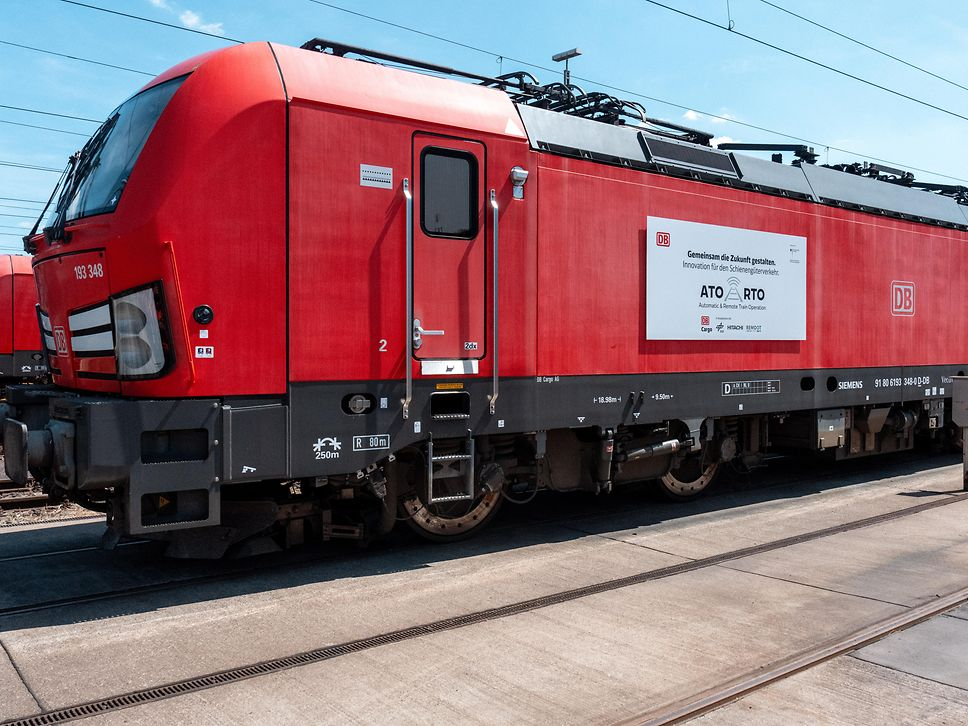
\includegraphics[width=0.7\textwidth]{vectron.jpg}
    \caption{Abgebildet ist eine der beiden Siemens-Vectron-Lokomotiven, die für die Datenerhebung eingesetzt wurden \cite{vectron}.}
    \label{fig:vectron}
\end{figure}

Der erfasste Datensatz erstreckt sich über einen kontinuierlichen Aufzeichnungszeitraum von 84 Tagen (Daten aus 2026) und umfasst ein Speichervolumen von circa 50 Gigabyte im komprimierten \texttt{pcapng.gz}-Format. 
Die Datenerfassung erfolgte über ein ethernet-basiertes Aufzeichnungssystem. 
Systembedingt unterliegen diese rohen Netzwerkdaten stark asynchronen Abtastraten: 
Aktorik-Signale wurden hochfrequent mit 20\,Hz aufgezeichnet, kinematische Größen mit 5\,Hz und statische Streckendaten mit lediglich bis zu 1\,Hz. 

Durch die formale Strukturierung lassen sich die extrahierten Roh-Variablen kategorisieren und den Dimensionen des Zustands- und Aktionsraums zuweisen. 
Die Fahrzeugkinematik wird durch die Ist-Geschwindigkeit (\texttt{V\_EST}) und die Beschleunigung (\texttt{A\_EST}) abgebildet. Die restriktiven Streckenlimits definieren sich über die erlaubten Zielgeschwindigkeiten (\texttt{V\_MRSP}, \texttt{V\_PERMITTED}). 
Ergänzt wird dieser Zustandsraum durch Topologie- und Kontextgrößen wie den Streckengradienten (\texttt{A\_GRADIENT}), die Schienenhaftung (\texttt{Q\_ADHESION}) und fahrzeuginterne Rückmeldungen (\texttt{M\_RST\_TBsetVal}). 
Dem gegenüber steht die Zielvariable \texttt{M\_ATO\_RTBRq} -- die vom menschlichen Fahrer geforderte Hebelstellung. Diese wird ausdrücklich als das Label $Y$ definiert, welches es zu prädizieren gilt. 
Durch diese präzise Zuweisung von Input-Features $X$ und Label $Y$ wird das unstrukturierte, reale Zug-Szenario mathematisch formalisiert und in ein klassisches Regressionsproblem des Supervised Learning ($X \rightarrow Y$) übersetzt.

Trotz dieser methodischen Fundierung weist der Datensatz a priori signifikante physikalische Limitationen auf, die offen adressiert werden müssen. 
Es liegt ausschließlich die Dynamik einer leeren Lokomotive vor; die immense Trägheit und die komplexe Wagendynamik eines schweren Güterzuges sind in diesen Daten nicht abgebildet. 
Ferner enthält der Datensatz fundamentale \textit{Hidden Variables} (unsichtbare Ereignisse) -- wie beispielsweise den direkten Sichtkontakt des Triebfahrzeugführers zu vorausliegenden Signalen oder Hindernissen, welche nicht im System protokolliert werden. 
Wenn das Modell in den Daten eine augenscheinlich grundlose Bremsung registriert, den wahren physikalischen Auslöser im Zustandsvektor jedoch nicht finden kann, entsteht das hochakademische Problem der \textit{Causal Confusion} (Ursachenverwechslung). 
Dieser Umstand erzeugt ein systematisches, nicht auflösbares Rauschen im Label, welches das Imitation Learning massiv erschwert, da das Netz gezwungen wird, diese Lücken mit potenziell falschen Korrelationen zu füllen.

\subsection{Explorative Datenanalyse und Bereinigung}

Bevor die historischen Rohdaten in formale Tensordarstellungen für das Training des neuronalen Netzes überführt werden können, ist eine systematische \gls{EDA} mit Datenbereinigung zwingend erforderlich. 
Künstliche neuronale Netze agieren fundamental als hochdimensionale, aber blinde Mustererkenner, die jegliche in den Eingangsdaten vorhandenen Korrelationen ungefiltert auf die Zielvariablen abbilden. 
Dies unterstreicht das fundamentale Paradigma des maschinellen Lernens „Garbage In, Garbage Out“, wonach fehlerhafte, verrauschte oder unvollständige Eingangsdaten unweigerlich zu dysfunktionalen und nicht generalisierbaren Prädiktionsmodellen führen.

In diesem Kontext fungiert die \gls{EDA} als essenzielles Diagnosewerkzeug. 
Sie dient dazu, systematisches Rauschen, Ausreißer und Anomalien in den realen Betriebsdaten frühzeitig zu identifizieren und durch geeignete Vorverarbeitungsschritte zu filtern. 
Durch diesen strengen Aufbereitungsprozess wird sichergestellt, dass das Modell im späteren Verlauf ausschließlich valide physikalische Kausalitäten der Zugsteuerung abstrahiert und nicht fälschlicherweise temporäre Sensorfehler oder Dateninkonsistenzen als gültige Fahrstrategie erlernt.

\subsubsection{Data Cleaning und zeitliche Synchronisierung}

Im ersten Schritt der Datenbereinigung müssen systemspezifische Fehlercodes, sogenannte Sentinels, sowie ungültige Messungen adressiert werden. 
Das Aufzeichnungssystem protokolliert Sensorausfälle durch fest definierte Extremwerte, wie beispielsweise $65535$ bei Geschwindigkeitssignalen (\texttt{V\_EST}, \texttt{V\_PERMITTED}) und $\pm 32768$ beziehungsweise $32767$ bei Beschleunigungs- und Gradientendaten (\texttt{A\_EST}, \texttt{A\_GRADIENT}). 
Diese artifiziellen Konstanten wurden konsequent durch \gls{NaN} ersetzt. 
Ergänzend erfolgte eine Out-of-Range-Maskierung, um physikalisch unmögliche Werte zu filtern. 
So wurden glitchbedingte Geschwindigkeitsspitzen von bis zu 371\,km/h eliminiert, wodurch sich ein realistisches Maximum von 141\,km/h bei einem 99,9-Perzentil von 125\,km/h einstellte. 
Nach dieser Bereinigung ergaben sich unterschiedliche Nutzbarkeitsquoten: 
Während essenzielle Signale und Labels (\texttt{V\_EST}, \texttt{M\_ATO\_RTBRq}, \texttt{M\_RST\_TBsetVal}, \texttt{M\_RST\_SlipSlide}) eine lückenlose Verfügbarkeit von 100\,\% aufwiesen, fiel diese bei \texttt{V\_PERMITTED}, \texttt{A\_EST} und \texttt{A\_GRADIENT} durch einen 11,49\,\%igen Sentinel-Ausfall auf 88,5\,\%. 
Stark ausgedünnt zeigten sich die Features \texttt{D\_STPDISTANCE} (38,2\,\% Nutzbarkeit aufgrund von 61,8\,\% fehlenden Werten) und \texttt{TOPO\_Q\_RADIUS} (35,1\,\%), was deren uneingeschränkte Nutzung limitiert.

Aus der Perspektive des maschinellen Lernens ist die Maskierung dieser Sentinels unerlässlich. 
Unmaskierte Extremwerte würden nachfolgende Skalierungsverfahren, wie die Min-Max- oder Z-Score-Normalisierung, vollständig dominieren, wodurch die reale Signalvarianz auf annähernd null gestaucht würde. 
Werden derart verzerrte Werte in das neuronale Netz gespeist, erzeugen sie extreme Aktivierungen im Forward-Pass. 
Dies führt unweigerlich zu verschwindenden oder explodierenden Gradienten (Vanishing/Exploding Gradients) und verhindert eine stabile Konvergenz des Modells während des Trainings.

Neben der Wertebereinigung erforderte die asynchrone und uneinheitliche Aufzeichnungsfrequenz der Rohdaten eine zeitliche Synchronisierung. 
Das ursprüngliche Median-Abtastintervall betrug circa 34\,ms, wies jedoch eine starke Spanne von 8 bis 118\,ms auf. 
Dies entspricht einer Übertragungsrate von etwa 28 bis 30\,Hz pro Signal, wobei jede Variable unabhängig getaktet war. 
Um eine verarbeitbare, konsistente Sequenzstruktur zu schaffen, wurden die Signalgruppen mittels Zeit-Binning und einem Outer-Join auf ein gemeinsames 200\,ms-Raster (5\,Hz) vereinheitlicht. 
Die durch diese Diskretisierung verbleibenden Datenlücken erwiesen sich als minimal: 
Der Median der größten Lücke pro Fahrt (Trip) lag bei lediglich 173\,ms. Lücken von über 2\,s existierten mit durchschnittlich 0,05 Vorkommnissen pro Trip praktisch nicht. 
Zur Sicherstellung der zeitlichen Kohärenz wurden Trips bei Unterbrechungen von mehr als 60\,s systematisch in separate Teilsequenzen getrennt.

Die Reduktion der zeitlichen Auflösung (Downsampling) von 30\,Hz auf 5\,Hz lässt sich physikalisch durch die immense Trägheit des Systems begründen. 
Aufgrund der hohen Zugmasse ändern sich Fahrzustände nur langsam, weshalb eine hochfrequente Abtastung eine erhebliche Überabtastung darstellt und keinen wesentlichen Informationsgewinn liefert. 
Durch das Downsampling wird die Rechenlast drastisch reduziert und die extrem hohe Autokorrelation benachbarter Frames minimiert, wodurch redundante Informationen aus dem Datensatz entfernt werden. 
Dies führt zu kompakteren Sequenzlängen, was insbesondere das \gls{BPTT}-Verfahren beim Training rekurrenter neuronaler Netze über lange zeitliche Horizonte signifikant stabilisiert.

\subsubsection{Analyse der Klassenverteilung}

Eine detaillierte Untersuchung der Werteverteilungen von Eingangsfeatures und Zielvariablen ist essenziell, um potenzielle Verzerrungen (Bias) im Modelltraining zu antizipieren. 
Abbildung \ref{fig:a_est_dist} illustriert exemplarisch die Verteilung des bereinigten Beschleunigungssignals \texttt{A\_EST} über den gesamten Datensatz. 
Auf der Abszisse sind die physikalischen Schätzwerte aufgetragen, während die Ordinate die absolute Häufigkeit der Vorkommnisse auf einer logarithmischen Skala darstellt. 
Die Verteilung zeigt eine deutliche Konzentration um den Nullpunkt, was die physikalische Realität der Trägheit und langer Phasen konstanter Geschwindigkeit im Schienenverkehr widerspiegelt.

\begin{figure}[htbp]
    \centering
    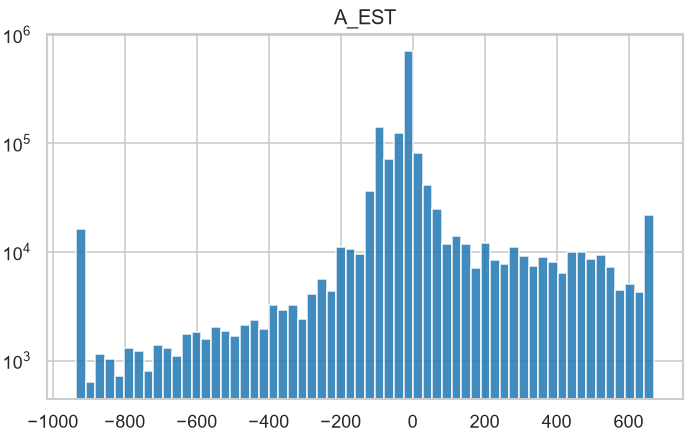
\includegraphics[width=0.8\textwidth]{02_distributions.png}
    \caption{Verteilung des Features \texttt{A\_EST} nach der Bereinigung. Die x-Achse zeigt die Signalwerte, die y-Achse die absolute Häufigkeit im Datensatz (logarithmische Skalierung).}
    \label{fig:a_est_dist}
\end{figure}

Analog zur Analyse der Eingangsfeatures wurde die Zielvariable, die Hebelstellung \texttt{M\_ATO\_RTBRq}, eingehend untersucht. 
Wie im linken Teildiagramm von Abbildung \ref{fig:label_dist} dargestellt, lässt sich das Fahrverhalten hinsichtlich der Aktionsrichtung in drei grundlegende Klassen unterteilen. 
Beschleunigungsphasen (Werte $> 0$) machen mit 49,2\,\% knapp die Hälfte der Daten aus. 
Bremsvorgänge (Werte $< 0$) repräsentieren 27,8\,\% der Aufzeichnungen. 
Die verbleibenden 23,0\,\% entfallen auf die exakte Neutralstellung beziehungsweise das Rollen des Zuges (Werte $= 0$). 
Das rechte Teildiagramm verdeutlicht ergänzend die Werteskalierung der aktiven Aktionen: 
Es zeigt sich, dass sich auch die tatsächlichen Hebelbewegungen stark um kleine Beträge nahe der Neutrallage konzentrieren und extreme Auslenkungen eher selten vorkommen.

\begin{figure}[htbp]
    \centering
    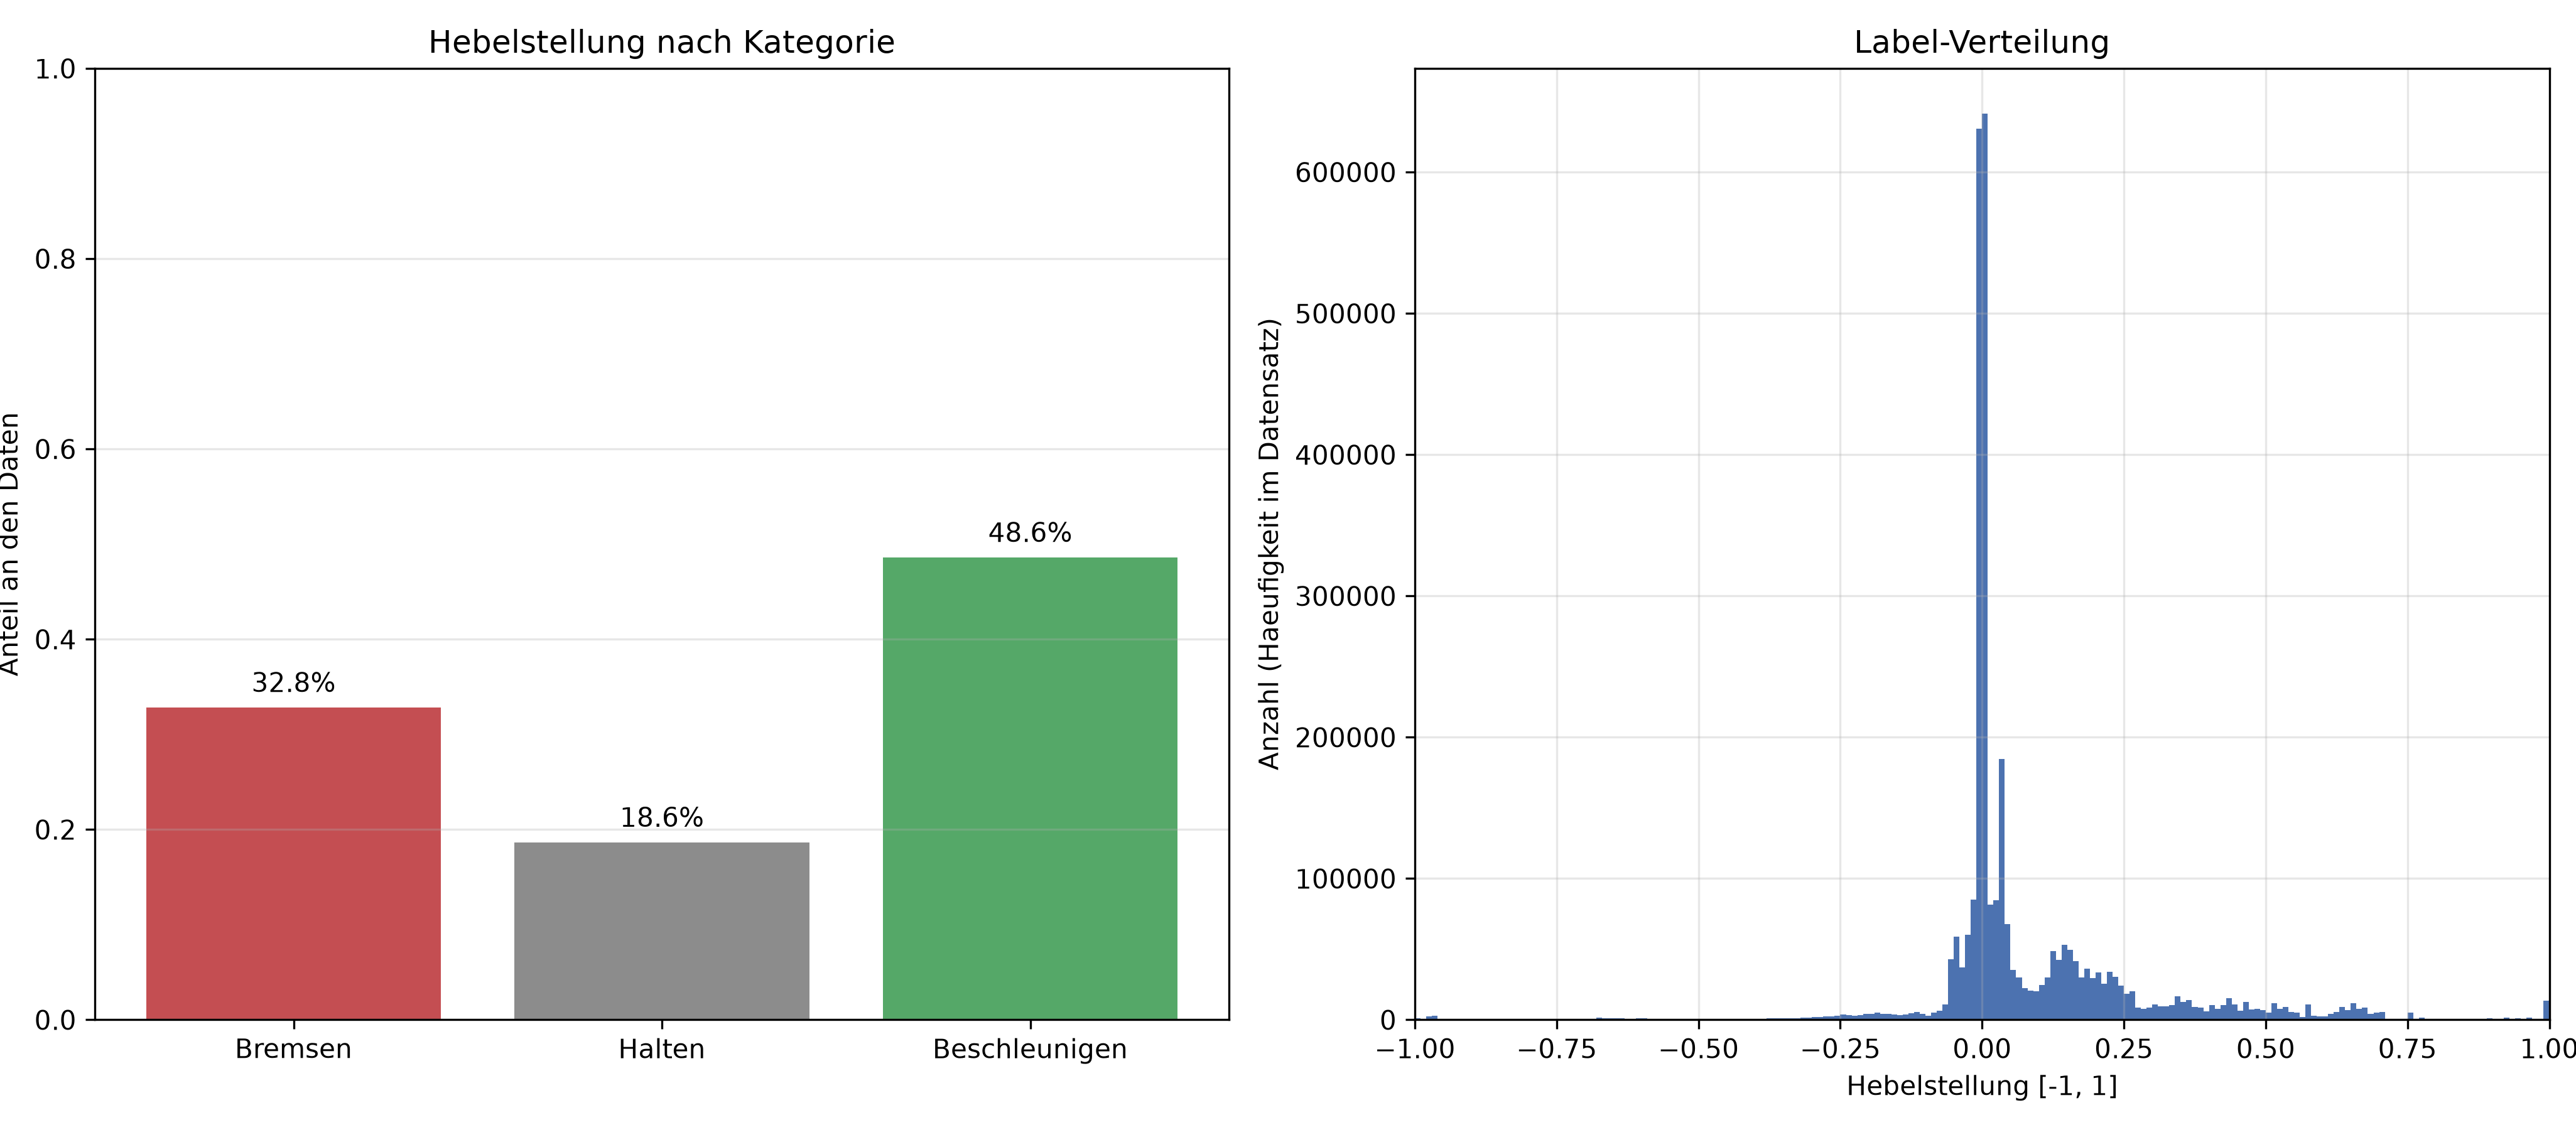
\includegraphics[width=1\textwidth]{07_label_analysis.png}
    \caption{Analyse der Zielvariable \texttt{M\_ATO\_RTBRq}. Links: Prozentuale Verteilung der diskreten Hebelzustände (Bremsen, Neutral, Beschleunigen). Rechts: Histogramm der kontinuierlichen Label-Werte (exklusive exakter Nullwerte), welches die starke Konzentration um kleine Beträge aufzeigt.}
    \label{fig:label_dist}
\end{figure}

Aus der Perspektive des maschinellen Lernens birgt diese ausgeprägte statistische Häufung von Null- und Quasi-Null-Aktionen ein erhebliches Risiko für den Optimierungsprozess, welches in der Literatur als Zero-Inflation-Problem beschrieben wird. 
Ein Anteil von 23\,\% exakt nullwertigen Labels in Kombination mit den dicht angrenzenden, minimalen Hebelstellungen verleitet das neuronale Netz dazu, in ein lokales Minimum zu konvergieren. 
Der Optimierungsalgorithmus tendiert in einem solchen Szenario dazu, ein „faules“ Modell zu formen, welches pauschal und konstant eine Hebelstellung von circa null prädiziert. 
Da der \gls{MSE} als klassische Verlustfunktion Ausreißer zwar stark bestraft, jedoch den Fehler über den gesamten Datensatz mittelt, erzeugt diese konstante Null-Prädiktion einen scheinbar niedrigen Gesamtfehler. 
Das Modell minimiert somit künstlich den Loss, ohne die tatsächlichen, kausalen Fahrdynamiken zu erlernen.

Um die Prädiktion einer rein statischen Roll-Strategie zu verhindern und das Modell zur aktiven, korrekten Handlung zu zwingen, muss diese konzeptionelle Unwucht zwingend in der späteren Trainingsphase adressiert werden. 
Das Problem erfordert gezielte Gegenmaßnahmen wie beispielsweise die Implementierung gewichteter oder asymmetrischer Loss-Funktionen, einen verstärkten Fokus auf isolierte Aktionsphasen während der Evaluierung oder die Anwendung balancierender Sampling-Strategien, um die Repräsentativität der relevanten Fahrentscheidungen im Trainingsdatensatz künstlich zu erhöhen.

\subsubsection{Korrelationsanalyse}

Um die statistischen Abhängigkeiten innerhalb des bereinigten Datensatzes zu quantifizieren und die Vorhersagekraft der einzelnen Sensordaten zu evaluieren, wurde eine Korrelationsanalyse durchgeführt. 
Die physikalischen Gesetzmäßigkeiten der Zugsteuerung -- beispielsweise das Verhältnis zwischen Bremskraft, Geschwindigkeit und Anhalteweg -- sind von ausgeprägten Sättigungseffekten und Nichtlinearitäten geprägt. 
Aus diesem Grund wurde für die Untersuchung der rangbasierte Spearman-Korrelationskoeffizient ($\rho$) gewählt. 
Im Gegensatz zur klassischen Pearson-Korrelation, welche ausschließlich lineare Zusammenhänge misst und nicht-lineare Effekte systematisch unterschätzen würde, erfasst die Spearman-Korrelation jegliche monotonen Beziehungen robust und verteilungsunabhängig. 
Die resultierende Korrelationsmatrix ist in Abbildung \ref{fig:spearman_corr} als Heatmap visualisiert.

\begin{figure}[htbp]
    \centering
    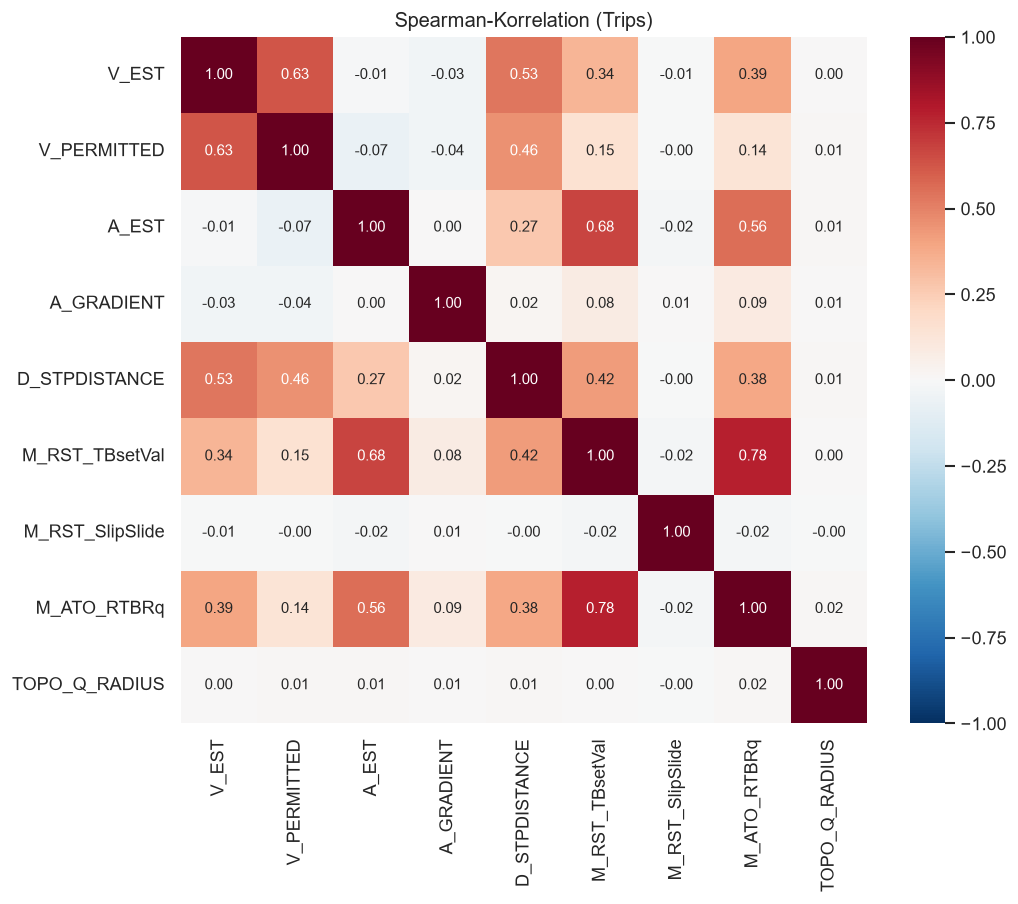
\includegraphics[width=1\textwidth]{05_spearman.png}
    \caption{Spearman-Korrelationsmatrix der Sensorwerte und der Zielvariable. Die Heatmap visualisiert die monotonen, nicht-linearen Abhängigkeiten zwischen den Features (Multikollinearität) sowie deren individuelle Vorhersagekraft für die Hebelstellung \texttt{M\_ATO\_RTBRq} (Feature Importance).}
    \label{fig:spearman_corr}
\end{figure}

Die Analyse der sogenannten Feature Importance, also der direkten Korrelation der Eingangsmerkmale mit der Zielvariable \texttt{M\_ATO\_RTBRq}, liefert essenzielle Erkenntnisse für die Modellbildung. 
Den stärksten Zusammenhang weist das Signal \texttt{M\_RST\_TBsetVal} mit $\rho = 0{,}78$ auf. 
Da es sich hierbei jedoch um die fahrzeugseitige Rückmeldung der real gestellten Kraft handelt, repräsentiert dieser Wert eine reaktive Größe, die extrem nah am prädiktiven Ziel selbst liegt. 
Die Verwendung dieses Features birgt ein hohes Risiko für Label-Leakage (das Modell erhält unbeabsichtigt die Lösung) und erfordert daher im weiteren Modellierungsverlauf höchste Vorsicht. 
Valide und signifikante prädiktive Zusammenhänge zeigen hingegen die geschätzte Beschleunigung \texttt{A\_EST} ($\rho = 0{,}56$), die Ist-Geschwindigkeit \texttt{V\_EST} ($\rho = 0{,}39$) sowie der Halteabstand \texttt{D\_STPDISTANCE} ($\rho = 0{,}38$), obgleich letzterer durch die zuvor beschriebene geringe Datenabdeckung von lediglich 38\,\% limitiert ist. 
Nur schwach korrelieren die zulässige Höchstgeschwindigkeit \texttt{V\_PERMITTED} ($\rho = 0{,}14$) und der Streckengradient \texttt{A\_GRADIENT} ($\rho = 0{,}09$). 
Die Variablen \texttt{M\_RST\_SlipSlide} ($\rho = -0{,}02$) und \texttt{TOPO\_Q\_RADIUS} ($\rho = 0{,}02$) erweisen sich hinsichtlich einer direkten monotonen Abhängigkeit als irrelevant für die Zielprädiktion.

Neben der Feature Importance offenbart die Matrix signifikante Interkorrelationen zwischen den unabhängigen Variablen, was auf eine ausgeprägte Multikollinearität hindeutet. 
Besonders hervorzuheben sind hierbei die starken Zusammenhänge zwischen \texttt{A\_EST} und \texttt{M\_RST\_TBsetVal} ($\rho = 0{,}68$) sowie innerhalb der kinematischen Metriken: \texttt{V\_EST} korreliert stark mit \texttt{V\_PERMITTED} ($\rho = 0{,}63$) und \texttt{D\_STPDISTANCE} ($\rho = 0{,}53$), während \texttt{V\_PERMITTED} und \texttt{D\_STPDISTANCE} ebenfalls eine deutliche Abhängigkeit aufweisen ($\rho = 0{,}46$).

Aus Perspektive des maschinellen Lernens ist diese Multikollinearität äußerst kritisch zu bewerten. 
Redundante, hochkorrelierte Variablen blähen den Merkmalsraum unnötig auf und begünstigen den Fluch der Dimensionalität (Curse of Dimensionality). 
Sie liefern dem neuronalen Netz keine zusätzliche Informationstiefe, sondern verstärken stattdessen das zugrundeliegende Datenrauschen und erhöhen das Risiko für Overfitting massiv. 
Zudem erschweren sie die Attributionsstabilität des Modells, da der Optimierungsalgorithmus beim Gradientenabstieg willkürlich die Gewichte zwischen den redundanten Features verschieben kann, ohne den Fehler (Loss) zu verändern. 
Folglich bilden diese stark korrelierenden Sensordaten primäre Kandidaten für eine systematische Entfernung oder Aggregation im anstehenden \gls{FE}.

\subsubsection{Physikalischer Plausibilitätscheck}

Um die funktionale Integrität des bereinigten Datensatzes abschließend zu verifizieren, wurde eine übergeordnete Plausibilitätsprüfung (Sanity-Check) anhand aggregierter Kennzahlen durchgeführt. 
Der Abgleich der geschätzten Sensor-Beschleunigung \texttt{A\_EST} mit der numerischen Ableitung der Geschwindigkeit nach der Zeit ($\frac{dV}{dt}$) ergab eine hohe Spearman-Korrelation von $\rho = 0{,}81$ bei einem Skalierungsfaktor von etwa $6$, was die physikalische Konsistenz der Sensorik bestätigt. 
Zudem stimmte das Vorzeichen der Hebelstellung in 78\,\% der Fälle mit der resultierenden Beschleunigungsrichtung überein. 
Auch die grundlegende Fahrlogik, wonach die Ist-Geschwindigkeit die zulässige Höchstgeschwindigkeit nicht überschreiten sollte (\texttt{V\_EST} $\le$ \texttt{V\_PERMITTED}), war in 90,7\,\% der Datenpunkte erfüllt. 
Physisch unmögliche Zustände wie negative Geschwindigkeiten (0\,\%) oder Werte über 150\,km/h traten nach der Bereinigung nicht mehr auf.

\begin{figure}[htbp]
    \centering
    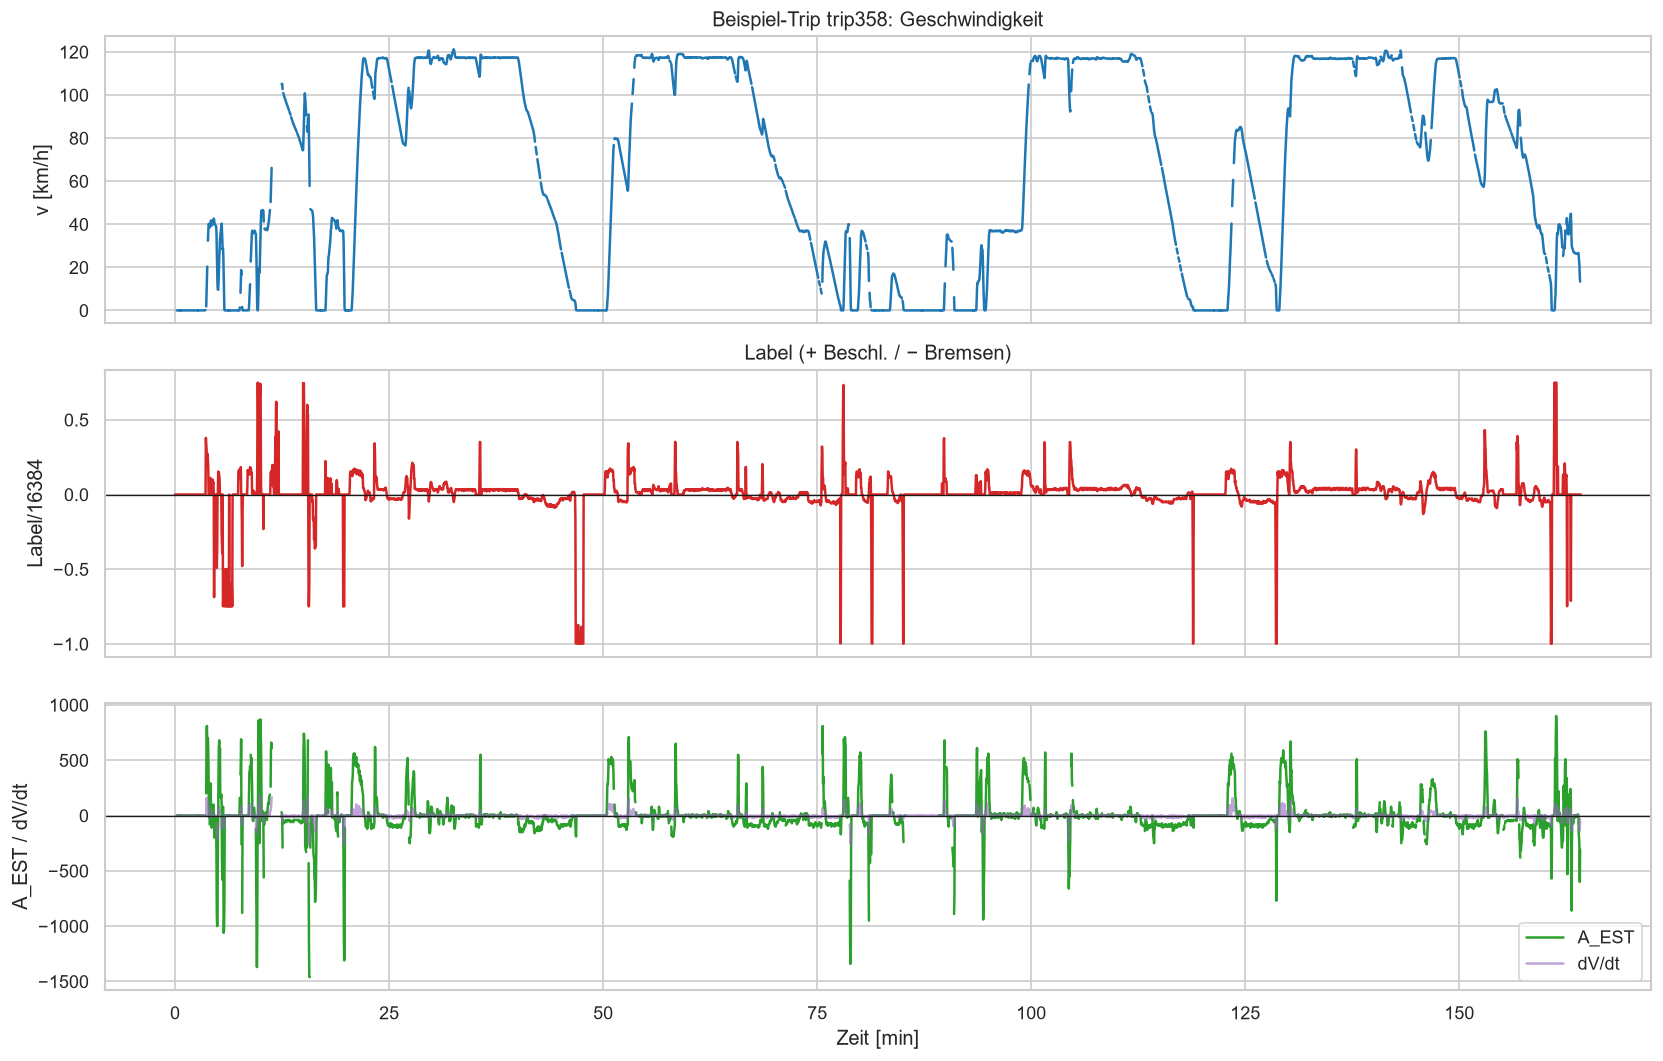
\includegraphics[angle=90,height=0.9\textheight]{11_sample_trip.png}
    \caption{Zeitreihen-Analyse einer beispielhaften Fahrt. Die Darstellung überlagert die physikalischen Zustandsgrößen (Geschwindigkeit und Beschleunigung) mit den korrespondierenden Expertenaktionen (Hebelstellung) über die Zeit und verdeutlicht das physikalisch plausible Brems- und Beschleunigungsverhalten.}
    \label{fig:sample_trip}
\end{figure}

Ergänzend zu den aggregierten Metriken bestätigt die visuelle Analyse einer exemplarischen Fahrt (siehe Abbildung \ref{fig:sample_trip}) die Kausalität des Fahrerverhaltens im Streckenkontext. 
Es zeigt sich deutlich, dass Bremsphasen (Label $< 0$) systematisch mit einer sinkenden Geschwindigkeit sowie einem abnehmenden Halteabstand (\texttt{D\_STPDISTANCE}) zusammenfallen. 
Das Beschleunigungsverhalten ist gleichermaßen nachvollziehbar, da der Zugkraftaufbau primär dann initiiert wird, wenn eine ausreichende Geschwindigkeitsreserve (Differenz zwischen \texttt{V\_PERMITTED} und \texttt{V\_EST}) vorhanden ist.

Trotz dieser offensichtlichen physikalischen Plausibilität offenbart die Analyse signifikante Lücken im Merkmalsraum. 
Wesentliche physikalische und umweltbedingte Einflussgrößen (Hidden Variables) sind im Datensatz nicht repräsentiert. 
Dazu zählen fundamentale fahrzeugspezifische Konstanten wie die aktuelle Zugmasse beziehungsweise Beladung, die Zuglänge sowie die exakte Bremskraft-Charakteristik des eingesetzten Fahrzeugtyps. 
Auch Umwelteinflüsse wie Nässe, Laub, Temperatur oder Wind, welche die Adhäsion massiv beeinflussen, fehlen gänzlich und lassen sich nur bedingt indirekt über das Radschlupf-Signal \texttt{M\_RST\_SlipSlide} erahnen. 
Darüber hinaus fehlt der übergeordnete betriebliche Kontext, wie etwa Zeitdruck durch den Fahrplan, vorausschauende Signalbilder aus der Linienzugbeeinflussung (LZB), die über das aktuelle \texttt{V\_PERMITTED} hinausgehen, oder der spezifische Grund eines Halts.

Aus der Perspektive des maschinellen Lernens stellen diese fehlenden Größen ein kritisches Problem beim Imitationslernen dar, welches als \textit{Causal Confusion} (Ursachenverwechslung) bezeichnet wird. 
Wenn ein Modell ausschließlich auf Expertenaktionen trainiert wird, deren wahre Auslöser es nicht „sehen“ kann, neigt es dazu, diese Aktionen mit stark korrelierenden, aber ursächlich falschen sichtbaren Variablen zu verknüpfen. 
Bremst ein Triebfahrzeugführer beispielsweise aufgrund nasser Schienen früher als gewöhnlich, erscheint dies für das Modell in Ermangelung von Wetterdaten als grundloses Bremsen bei einer bestimmten Geschwindigkeit. 
Das Modell erlernt somit eine fehlerhafte Kausalität. 
Um das Risiko zu minimieren, dass die Policy derartige Scheinkorrelationen adaptiert, müssen diese Faktoren im weiteren Forschungsverlauf - etwa durch gezielte Feature-Anreicherung oder die Integration von Unsicherheitsmodellierungen - adressiert werden.

\subsection{Feature Engineering}

Nach der initialen Bereinigung und Analyse der historischen Rohdaten bildet das domänenspezifische \gls{FE} den nächsten methodischen Schritt. 
Rohe Sensordaten allein bilden die zugrundeliegenden physikalischen Kausalitäten der Zugsteuerung oft nicht in einer Form ab, die von einem maschinellen Lernmodell effizient extrahiert werden kann. 
Um dem neuronalen Netz die komplexe Fahrentscheidung zu erleichtern und das Risiko von Kausalitätsfehlern zu minimieren, müssen die Eingangsdaten gezielt durch physikalisch motivierte, abgeleitete Merkmale ergänzt werden. 
Dieser Prozess transformiert implizites Systemwissen in explizite numerische Features, wodurch das Modell befähigt wird, vorausschauende statt rein reaktive Fahrstrategien zu erlernen.

\subsubsection{Methodik und Evaluierung}

Ein zentraler Aspekt bei der Konstruktion und Auswahl potenzieller Eingangsmerkmale ist die strikte Prävention von sogenanntem Label-Leakage. 
Wie die vorangegangene Korrelationsanalyse offenbarte, weist das rohe Feature \texttt{M\_RST\_TBsetVal} -- die fahrzeugseitige Rückmeldung der tatsächlich gestellten Kraft -- mit $\rho = 0{,}78$ die stärkste Spearman-Korrelation zur Zielvariable auf. 
Trotz dieser enorm hohen prädiktiven Kraft darf dieses Signal unter keinen Umständen als Feature für das Modelltraining herangezogen werden. 
Aus der Perspektive des maschinellen Lernens würde die Inklusion dieses Wertes zu einem gravierenden Informationsleck führen. 
Das neuronale Netz würde nicht die kausalen physikalischen Zusammenhänge der Streckentopologie erlernen, sondern lediglich die bereits vom Fahrzeug berechnete Rückmeldung trivial abschreiben, da diese der Zielvariable \texttt{M\_ATO\_RTBRq} naturgemäß stark ähnelt. 
Das Modell würde die Lösung somit bereits während der Vorhersage präsentiert bekommen (Label-Leakage).

Um eine konsistente zeitliche Basis für das Feature Engineering zu gewährleisten, erfolgt die Berechnung aller abgeleiteten Merkmale iterativ pro Fahrt (Trip) auf dem etablierten 200-ms-Raster. 
Für zeitliche Glättungen und Ableitungen werden dabei gleitende Fenster (Rolling Windows) von zehn Samples genutzt, was einem physikalischen Zeitraum von etwa zwei Sekunden entspricht.

Zur systematischen und objektiven Bewertung der Relevanz neu generierter Features wird eine Tri-Metrik-Evaluation angewendet. 
Da ein einzelnes statistisches Maß die komplexen Zusammenhänge in hochdimensionalen und multikollinearen Daten oft nur unzureichend oder verzerrt abbildet, werden drei komplementäre Evaluationsmetriken herangezogen:

\begin{itemize}
    \item \textbf{Absoluter Spearman-Koeffizient ($|\rho|$):} Diese Metrik misst robuste, monotone -- und damit auch nicht-lineare -- Zusammenhänge zwischen dem jeweiligen potenziellen Feature und der Zielvariable.
    \item \textbf{Mutual Information (MI):} Dieses informationstheoretische Maß erfasst jegliche Form von Abhängigkeiten, einschließlich rein nicht-linearer und nicht-monotoner Informationsgehalte, die durch klassische Korrelationskoeffizienten nicht abgebildet werden.
    \item \textbf{Absoluter standardisierter OLS-Koeffizient ($|\beta|$):} Mittels einer gewöhnlichen Fehlerquadratmethode (Ordinary Least Squares, OLS) wird der tatsächliche multivariate Beitrag eines Features bewertet, wobei die Effekte bestehender Multikollinearität systematisch herausgerechnet werden.
\end{itemize}

Durch die Kombination dieser drei Betrachtungswinkel lässt sich die Prädiktionsgüte jedes konstruierten Merkmals ganzheitlich quantifizieren, bevor es in den finalen Feature-Vektor des neuronalen Netzes aufgenommen wird.

\subsubsection{Kinematische Features}

Die erste Kategorie des \gls{FE} fokussiert sich auf die Bewegungsdynamik des Schienenfahrzeugs. 
Ziel ist es, aus den teils stark verrauschten rohen Geschwindigkeits- und Beschleunigungsdaten verlässliche Prädiktoren zu extrahieren, welche die tatsächliche Kinematik für das neuronale Netz optimal abbilden. 

Das aussagekräftigste Merkmal dieser Kategorie -- und gleichzeitig der Gesamtsieger der Evaluation (Rang 1) -- ist die zeitlich geglättete Beschleunigung \texttt{a\_est\_roll\_mean\_2s}. 
Sie berechnet sich als der gleitende Mittelwert (Simple Moving Average) des rohen Beschleunigungssignals über ein Fenster von zwei Sekunden ($n = 10$ Zeitschritte im 200-ms-Raster):

\begin{equation}
    a_{\text{est\_roll\_mean\_2s}, t} = \frac{1}{n} \sum_{i=0}^{n-1} a_{\text{est}, t-i} \quad \text{mit} \quad n=10
\end{equation}

Aus Sicht des maschinellen Lernens wirkt diese Operation wie ein essenzieller Tiefpassfilter. 
Das sprunghafte und von Sensorrauschen geprägte Originalsignal \texttt{A\_EST} wird entrauscht, wodurch der zugrundeliegende physikalische Trend maschinell verdaubar wird. 
Dies spiegelt sich in den hervorragenden Evaluationsmetriken wider: Das Feature erreicht einen Spearman-Koeffizienten von $0{,}52$ und die höchste Mutual Information (MI) von $0{,}26$.

Als ergänzendes Feature wurde die numerische Ableitung der Ist-Geschwindigkeit nach der Zeit, \texttt{a\_num} ($\frac{dV}{dt}$), berechnet (Rang 3). 
Die Berechnung über das diskrete Zeitintervall $\Delta t = 0{,}2\,\text{s}$ lautet:

\begin{equation}
    a_{\text{num}, t} = \frac{v_{\text{est}, t} - v_{\text{est}, t-1}}{\Delta t}
\end{equation}

Obwohl dieses Merkmal eine starke monotone Beziehung zur Zielgröße aufweist (Spearman $0{,}43$), zeigt die ML-Bewertung Schwächen im multivariaten Kontext. 
Numerische Ableitungen realer Sensordaten sind prinzipbedingt ausreißerbehaftet. 
Zudem sinkt der standardisierte OLS-Koeffizient auf $|\beta| = 0{,}15$, da \texttt{a\_num} stark kollinear (redundant) zur bereits vorhandenen Sensor-Beschleunigung \texttt{A\_EST} ist und dem Modell somit nur begrenzten multivariaten Mehrwert liefert.

Ein Paradebeispiel für die Notwendigkeit der Tri-Metrik-Evaluation liefert das Feature \texttt{v\_roll\_std\_2s} (Rang 6). 
Es beschreibt die gleitende Standardabweichung der Geschwindigkeit über ein Zwei-Sekunden-Fenster und quantifiziert die lokale Volatilität der Fahrt:

\begin{equation}
    v_{\text{roll\_std\_2s}, t} = \sqrt{\frac{1}{n-1} \sum_{i=0}^{n-1} \left( v_{\text{est}, t-i} - \bar{v}_{\text{est}, (t, n)} \right)^2} \quad \text{mit} \quad n=10
\end{equation}

Die lineare und monotone Korrelation dieses Features mit der Zielvariable ist praktisch null (Spearman $\approx 0$). 
Die Mutual Information erreicht jedoch einen signifikanten Wert von $0{,}15$. 
Dieses Merkmal fungiert für das Modell als ein rein nicht-linearer Indikator für volatile Phasen, beispielsweise an den kritischen Übergängen zwischen Brems- und Beschleunigungsvorgängen, was von klassischen Korrelationsmetriken völlig unbemerkt bliebe.

Als am wenigsten geeignet (Rang 6,3) erwies sich hingegen der Ruck (\texttt{jerk}), welcher die zeitliche Änderungsrate der Beschleunigung darstellt:

\begin{equation}
    jerk_t = \frac{a_{\text{num}, t} - a_{\text{num}, t-1}}{\Delta t}
\end{equation}

Die physikalische und mathematische Natur dieses Features verdeutlicht eine fundamentale Grenze beim Feature Engineering mit realen Betriebsdaten. 
Als zweite numerische Ableitung des ohnehin leicht verrauschten Geschwindigkeitssignals degeneriert das Signal-Rausch-Verhältnis vollständig. Das resultierende Feature besteht fast ausschließlich aus hochfrequentem Rauschen, bietet dem neuronalen Netz keinerlei stabilen prädiktiven Mehrwert und verschlechtert potenziell die Robustheit der Policy.

\subsubsection{Kontext- und Regelabweichungs-Features}

Neben der reinen Bewegungsdynamik erfordert eine vorausschauende Fahrstrategie die situative Einordnung des Schienenfahrzeugs im betrieblichen Umfeld. 
Die nachfolgenden Merkmale quantifizieren die fortlaufende Regelabweichung, indem sie den aktuellen physikalischen Fahrzustand in Relation zu den deterministischen Streckenvorgaben -- insbesondere zu Geschwindigkeitsbegrenzungen und Haltepunkten -- setzen. 
Das neuronale Netz muss "wissen", wie nah sich der Zug an seinen operationellen Limits und Zielen befindet.

Das effektivste Merkmal dieser Kategorie und das zweitbeste Feature der Gesamtauswertung (Rang 2) ist die relative Ausnutzung des zulässigen Geschwindigkeitslimits, definiert als \texttt{v\_ratio}:

\begin{equation}
    v_{\text{ratio}, t} = \frac{v_{\text{est}, t}}{v_{\text{permitted}, t}}
\end{equation}

Aus Sicht des maschinellen Lernens erweist sich dieser Quotient als das mit Abstand beste Kontext-Feature. 
Durch die mathematische Normierung ist die Größe intrinsisch skaliert und gegenüber absoluten Geschwindigkeitsschwankungen äußerst robust. 
Dieser Informationsgehalt schlägt sich in einem extrem hohen multivariaten Beitrag nieder, welcher durch einen standardisierten OLS-Koeffizienten von $|\beta| = 0{,}21$ quantifiziert wird. 
Das Modell lernt aus dieser Größe unmittelbar, wie viel Spielraum bis zum zwingenden Bremseingriff der Zugbeeinflussungssysteme verbleibt.

Ergänzend zur relativen Metrik wurde die absolute Geschwindigkeitsreserve \texttt{v\_headroom} berechnet (Rang 4,7):

\begin{equation}
    v_{\text{headroom}, t} = v_{\text{permitted}, t} - v_{\text{est}, t}
\end{equation}

Die Evaluation dieses Features veranschaulicht eindrucksvoll die Problematik der Multikollinearität im Feature Engineering. 
Univariat betrachtet ist das Merkmal äußerst aussagekräftig, was durch einen hohen Mutual-Information-Wert (MI) von $0{,}29$ belegt wird. 
Im multivariaten Kontext des Modells fällt die Relevanz jedoch signifikant ab ($|\beta| = 0{,}08$). 
Die Ursache hierfür liegt in der massiven Redundanz zu \texttt{v\_ratio} und den zugrundeliegenden rohen Geschwindigkeitssignalen. 
Das Merkmal bläht den Merkmalsraum auf, ohne dem Netz unabhängige, neue Informationen zu liefern.

Zur Modellierung des zielgenauen Bremsverhaltens vor Bahnhöfen oder Signalen wurde das Merkmal \texttt{stop\_proximity} entworfen (Rang 5). 
Um eine Singularität bei Erreichen des Zielpunktes ($D = 0$) zu vermeiden, wird die inverse Distanz unter Addition einer Konstanten berechnet:

\begin{equation}
    \text{stop\_proximity}_t = \frac{1}{|D_{\text{STPDISTANCE}, t}| + 1}
\end{equation}

ML-theoretisch und physikalisch stellt diese nicht-lineare Transformation einen brillanten Bremsindikator dar. 
Der Wert verharrt auf langen Streckenabschnitten nahe null und steigt exakt in der kritischen Phase kurz vor dem Haltepunkt exponentiell an, was dem Modell ein klares, starkes Signal für den Bremseinsatz liefert. 
Die praktische Nutzbarkeit in diesem spezifischen Anwendungsfall wird jedoch durch ein fundamentales Datenproblem stark limitiert: 
Wie die explorative Datenanalyse ergab, weist das zugrundeliegende Rohsignal \texttt{D\_STPDISTANCE} lediglich eine nutzbare Abdeckung (Coverage) von 38\,\% auf. 
Ein Modell, das bei der Prädiktion der Bremskurve ein hohes Gewicht auf dieses Feature legt, würde in den restlichen 62\,\% der Fälle mangels Sensordaten scheitern.

\subsubsection{Engineered Feature Pruning}

Um die Erkenntnisse der Tri-Metrik-Evaluation zusammenzuführen und den finalen Eingangsvektor für das neuronale Netz zu definieren, werden die berechneten Wichtigkeiten in Abbildung \ref{fig:engineered_importance} visuell gegenübergestellt. 
Die Darstellung veranschaulicht eindrucksvoll die Notwendigkeit mehrerer Evaluierungsansätze: 
Insbesondere die Divergenz zwischen der Spearman-Korrelation und der Mutual Information (MI) offenbart wertvolle, rein nicht-lineare Zusammenhänge, die von klassischen Korrelationsmaßen ignoriert werden, wie es signifikant bei der gleitenden Geschwindigkeitsstreuung (\texttt{v\_roll\_std\_2s}) der Fall ist.

\begin{figure}[htbp]
    \centering
    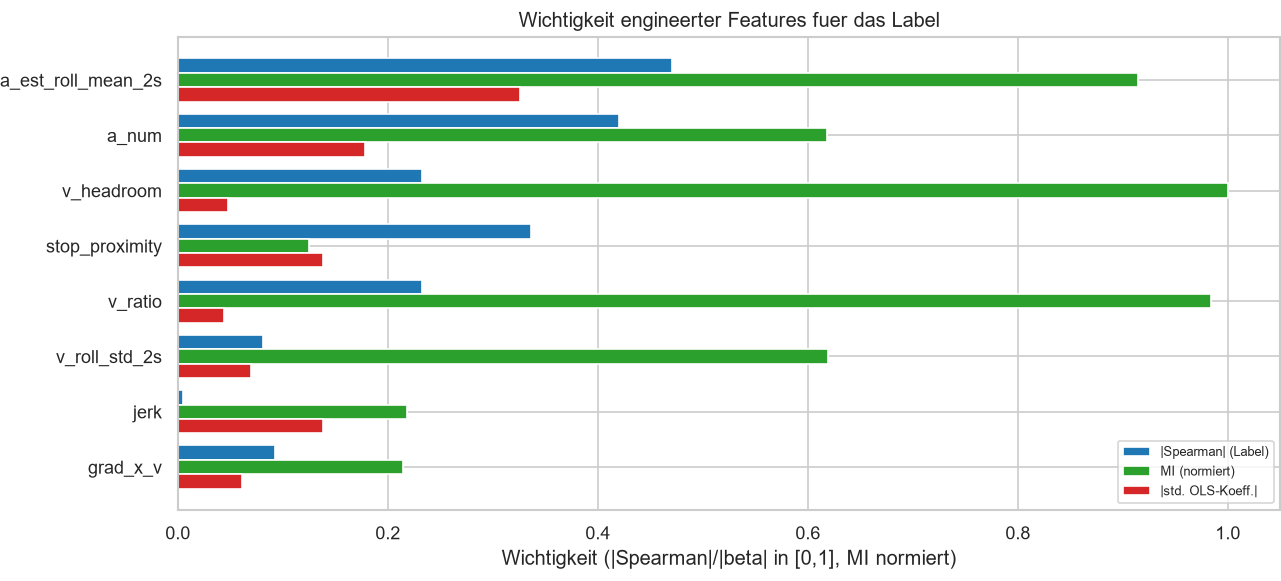
\includegraphics[width=1\textwidth]{06_engineered_importance.png}
    \caption{Vergleich der Feature-Wichtigkeit anhand dreier komplementärer Metriken. Die Divergenz zwischen Spearman-Korrelation und Mutual Information (MI) offenbart rein nicht-lineare Zusammenhänge (z.\,B. bei \texttt{v\_roll\_std\_2s}).}
    \label{fig:engineered_importance}
\end{figure}

Basierend auf dieser quantitativen Datenlage erfolgt das abschließende Feature Pruning. 
In diesem Schritt werden gezielt Variablen aus dem Datensatz entfernt, die keinen unabhängigen Mehrwert liefern oder die numerische Stabilität des Trainings gefährden. 
Konsequent verworfen werden hochgradig redundante Merkmale wie die absolute Geschwindigkeitsreserve \texttt{v\_headroom}, deren Informationsgehalt bereits durch die robustere und normierte relative Ausnutzung \texttt{v\_ratio} abgedeckt ist. Ebenso
 werden stark verrauschte oder prädiktiv unbedeutende Variablen, darunter der Ruck (\texttt{jerk}) sowie weitere experimentelle Kreuzterme wie \texttt{grad\_x\_v}, aus dem finalen Merkmalsraum ausgeschlossen.

Aus der Perspektive des maschinellen Lernens ist dieser Reduktionsschritt essenziell. 
Die bewusste Konzentration auf ein schlankes Modell mit weitestgehend orthogonalen, also mathematisch unabhängigen, Features verhindert effektiv den Fluch der Dimensionalität (Curse of Dimensionality). 
Ein kompakter, informationsdichter Zustandsraum entlastet den Optimierungsalgorithmus und reduziert die Gefahr irrelevanter Parameteranpassungen. 
Vor allem minimiert diese Strenge bei der Merkmalsauswahl das im Offline-Imitationslernen omnipräsente Risiko des Overfittings, da dem neuronalen Netz signifikant weniger Rauschquellen und Scheinkorrelationen zur fälschlichen Überanpassung (Memorization) zur Verfügung gestellt werden.
    \newpage

    \section{Konzeption der Modellarchitektur}
\label{ch:konzeption_modellarchitektur}

Aufbauend auf der systematischen Transformation des unstrukturierten Rohdatensatzes in einen maschinenlesbaren Zustandsraum erfolgt in diesem Kapitel die informationstechnische Konzeption der neuronalen Modellarchitektur. 
Das primäre methodische Ziel besteht in der Konstruktion einer Policy $\pi_\theta$, welche in der Lage ist, auf Basis historischer Zeitreihen einen kontinuierlichen Aktionsraum -- spezifisch die Leistungs- und Bremshebelstellung -- prädiktiv abzubilden. 

\subsection{Auswahlder Architektur}
\label{sec:auswahl_architektur}

Um eine fundierte Entscheidung für die finale Modellstruktur zu treffen, wurde ein initiales experimentelles Setup aufgesetzt. 
In dieser Evaluationsphase wurden ein \acrlongshort{MLP}, ein \acrlongshort{LSTM} sowie eine \acrlongshort{GRU} vergleichend trainiert und analysiert.

\subsubsection{Experimentelles Setup}
Die initiale Trainingsphase wurde bewusst ohne Regularisierungsmaßnahmen wie Dropout oder Weight Decay (L2-Regularisierung) durchgeführt. 
Dieses Vorgehen stellt sicher, dass das native Lernverhalten sowie die prinzipielle Eignung der Architekturtypen für die Verarbeitung fahrphysikalischer Zeitreihen isoliert betrachtet werden können. 
Für eine effiziente Evaluation wurde das Training auf 20\,\% des Gesamtdatensatzes limitiert und über 10 Epochen mit einer Batch-Size von 256 sowie einer Learning Rate von 0.001 ausgeführt. 
Das Eingangsfenster umfasste 100 Zeitschritte ($H=100$), was physikalisch 20 Sekunden an historischen Daten entspricht, um einen Vorhersagehorizont von 50 Zeitschritten (10 Sekunden) zu prädizieren.

Die Auswertung des Feedforward-Netzwerkes verdeutlicht die theoretischen Limitationen dieser Architektur. 
Mit 110.849 trainierbaren Parametern wies das \gls{MLP} die massivste Überdimensionierung im Testfeld auf und erreichte konsequenterweise den geringsten Trainingsfehler (siehe Abbildung \ref{fig:training_loss_comparison}). 
Auf den ungesehenen Evaluierungsdaten versagte das Modell jedoch: 
Der Validierungs-\gls{RMSE} lag bei 0.2297 (\gls{MAE} = 0.1476), und das Bestimmtheitsmaß auf dem Test-Set fiel auf ein $R^2$ von lediglich 0.0467 bei einer Richtungs-Accuracy von 47,52\,\% und einer Toleranz-Accuracy von 70,57\,\%. 

Aus maschineller Lernperspektive handelt es sich hierbei um ein klassisches Phänomen der extremen Überanpassung (Overfitting). 
Wie in den theoretischen Grundlagen hergeleitet, besitzen Feedforward-Netze keinen internen Zustand (Hidden State) und verarbeiten Eingaben rein statisch. 
Sie sind nicht in der Lage, zeitliche Kausalitäten -- wie die immense physikalische Trägheit eines Zuges -- zu erfassen. 
Das \gls{MLP} nutzt seine enorme Parameteranzahl folglich ausschließlich zur reinen Memorization (Auswendiglernen) der Trainingsdaten. 
Sobald das Modell auf ungesehene Evaluierungsdaten trifft, fehlt ihm das temporale Verständnis, was zu einer Explosion des Validierungs-Losses führt.

Im direkten Kontrast dazu demonstrierten die rekurrenten Architekturen eine deutliche Überlegenheit. 
Das \gls{LSTM} (19.009 Parameter) erzielte ein Test-$R^2$ von 0.1030 bei einem \gls{RMSE} von 0.1550 und einem \gls{MAE} von 0.0898. 
Die Richtungs-Accuracy stieg auf 60,95\,\% (Toleranz-Accuracy: 73,55\,\%). 
Die \gls{GRU} (14.273 Parameter) lieferte ähnliche, minimal schwächere Metriken mit einem Test-$R^2$ von 0.0854 (\gls{RMSE} = 0.1565, \gls{MAE} = 0.0864) und einer Richtungs-Accuracy von 60,85\,\%.

\begin{figure}[htbp]
    \centering
    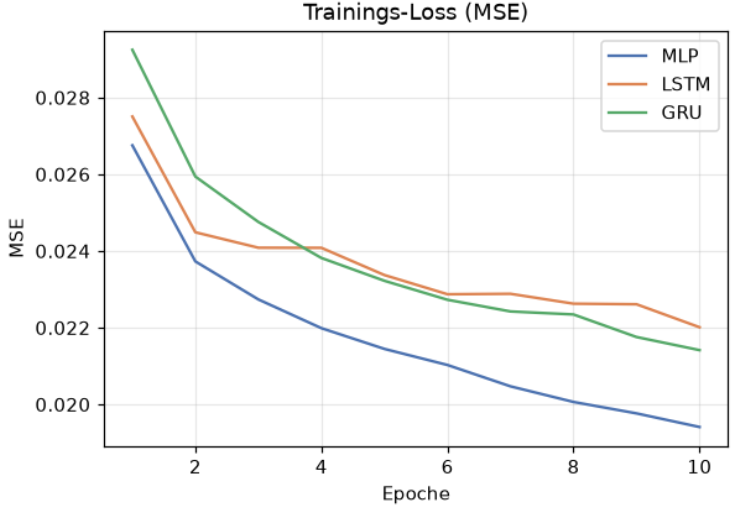
\includegraphics[width=\textwidth]{loss_comparison.png}
    \caption[Trainings- und Validierungsverluste]{Vergleich der Trainings- und Validierungsverluste der evaluierten Basis-Architekturen zur Visualisierung des architekturabhängigen Lernverhaltens.}
    \label{fig:training_loss_comparison}
\end{figure}

Diese Ergebnisse belegen die Theorie: 
\gls{LSTM} und \gls{GRU} glänzen, da sie exakt für derartige hochgradig sequenzielle Aufgaben entworfen wurden. 
Durch ihre rekurrente Architektur und die spezialisierten Gating-Mechanismen (wie den Cell State beim \gls{LSTM}) können sie historische Abhängigkeiten über das gesamte 20-sekündige Eingangsfenster aggregieren. 
Das Modell begreift mathematisch, dass ein aktuelles Bremsmanöver kausal mit infrastrukturellen oder physikalischen Signalen aus der Vergangenheit zusammenhängt.

Ein wissenschaftlich interessantes Phänomen zeigte sich zudem bei den Trainingszeiten. 
Aus informationstheoretischer Sicht sollte die \gls{GRU} recheneffizienter agieren, da sie durch die Einsparung von Gates mit lediglich 14.273 Parametern deutlich schlanker ist als das \gls{LSTM} (19.009 Parameter). 
Dennoch beanspruchte das Training der \gls{GRU} 654,8 Sekunden, während das \gls{LSTM} bereits nach 399,7 Sekunden konvergierte.

Diese Laufzeit-Anomalie lässt sich durch die zugrundeliegende Software-Architektur erklären. 
In etablierten Deep-Learning-Frameworks wie PyTorch wurden die Implementierungen von \gls{LSTM}-Zellen über Jahre hinweg auf Hardware- und C++-Ebene extrem stark optimiert. 
Die internen Matrixmultiplikationen der \gls{LSTM}-Zellen lassen sich oftmals effizienter parallelisieren als die strikt sequenziellen Update-Schritte der \gls{GRU}. 
Diese hochgradige Software-Optimierung überwiegt in der Praxis den theoretischen Rechenvorteil der geringeren Parameterzahl bei Weitem.

\subsubsection{Fazit der Architekturauswahl}

Unter Berücksichtigung der fundamentalen Anforderungen an die Generalisierungsfähigkeit fällt die finale Entscheidung -- trotz des minimal stärkeren Test-$R^2$ des \glsentryshort{LSTM}s im initialen Setup -- auf die \gls{GRU}-Architektur. 
Aus maschineller Lernperspektive bietet die \gls{GRU} durch ihre reduzierte Parameterzahl einen entscheidenden strukturellen Vorteil: Eine geringere Modellkapazität verringert nativ die Anfälligkeit für Overfitting und zwingt das Netzwerk dazu, robustere, abstrahierte Repräsentationen der Fahrphysik zu erlernen. 
Der im Vorfeld identifizierte Laufzeitnachteil der \gls{GRU}, welcher auf PyTorch-spezifische Implementierungsdetails zurückzuführen ist, ist für den weiteren Projektverlauf zu vernachlässigen, da das finale und rechenintensive Modelltraining ohnehin auf einer deutlich leistungsstärkeren Hardware-Infrastruktur durchgeführt wird. 
Da jedoch auch die \gls{GRU} als unregularisiertes Basis-Modell nicht vollständig immun gegen das Auswendiglernen von Trajektorien ist, ist die Definition und Implementierung fundierter Regularisierungsstrategien für die Konstruktion der finalen Policy zwingend erforderlich.

\subsection{Dimensionierung des Netzwerks}
\label{subsec:dimensionierung_netzwerk}

Die Dimensionierung eines neuronalen Netzes unterliegt einem fundamentalen informationstheoretischen Dilemma: 
Eine zu geringe Modellkapazität bedingt Underfitting, wodurch die komplexe Zugdynamik nicht ausreichend abgebildet werden kann. 
Eine zu große Architektur neigt hingegen -- insbesondere bei verrauschten realen Sensordaten -- zu starkem Overfitting, da das Modell den Trainingsdatensatz auswendig lernt (Memorization) und seine Generalisierungsfähigkeit einbüßt. 
Um das optimale Gleichgewicht empirisch zu ermitteln, wurde ein Brute-Force-Grid-Search-Verfahren implementiert. 
Hierbei wurden 39 permutationsfähige Architekturen des ausgewählten \gls{GRU}-Modells mit einer Tiefe von ein bis drei Hidden Layern und Breiten von 64, 96 sowie 128 Neuronen unter identischen Bedingungen (10 Epochen, Batch-Size 128, Learning Rate 0.001) trainiert. 
Als finale Entscheidungsmetrik diente der \acrlongshort{MSE} auf dem isolierten Test-Datensatz.

Die empirische Evaluation der Single-Layer-Architekturen offenbarte das schlechteste Leistungsniveau. 
Dies belegt, dass ein einzelner rekurrenter Layer nicht über die notwendige Repräsentationskapazität verfügt, um die hochdimensionalen Abstraktionen zwischen Streckentopologie, Kinematik und resultierender Hebelstellung über das definierte Zeitfenster ($H=30$) zu erlernen. 
Eine Erhöhung der Tiefe auf drei Hidden Layer (mit bis zu 251.265 Parametern) verschlechterte die Prädiktionsgüte jedoch massiv. 
Diese tiefen Modelle unterliegen starkem Overfitting, da sie aufgrund der enormen Parameterzahl streckenspezifische Eigenheiten und Sensorrauschen memorieren, anstatt die kausale Fahrphysik zu generalisieren.

Das globale Optimum des Experiments verortet sich in den 2-Layer-Architekturen, welche im Durchschnitt den geringsten Test-Fehler (0.0205) aufweisen. 
Als beste Einzelkonfiguration kristallisierte sich ein Netzwerk mit 96 Neuronen im ersten und 64 Neuronen im zweiten Hidden Layer heraus (Test-\gls{MSE}: 0.0197 bei 61.697 Parametern). 
Das finale Modell für das \gls{BC} wird folglich als 2-Layer-\gls{GRU} mit dieser asymmetrischen Trichterstruktur (Funnel-Design) dimensioniert. 
Dieses Layout ist konzeptionell äußerst vorteilhaft: Der breitere erste Layer extrahiert komplexe, hochfrequente zeitliche Kausalitäten aus dem acht-dimensionalen Input-Strom. 
Der darauffolgende, schmalere Layer agiert als ,,Information Bottleneck''. 
Er zwingt das Modell, die extrahierten Informationen auf die essenziellen physikalischen Treiber zu komprimieren, bevor die finale Vorhersageschicht den kontinuierlichen Stellwert generiert. 
Dieses Design bietet das ideale Verhältnis aus Repräsentationskapazität und inhärenter Regularisierung.

\subsection{Loss-Funktion und Optimizer}
\label{subsec:loss_und_optimizer}

Die finale Prädiktionsgüte der neu ausgewählten 2-Layer-\gls{GRU}-Architektur (96-64 Neuronen) wird im hochdimensionalen Parameterraum maßgeblich von der mathematischen Fehlerbewertung (Verlustfunktion) sowie der algorithmischen Optimierungsstrategie determiniert. 
Um die optimale Konfiguration für diese tiefe Netzwerkstruktur zu ermitteln, wurde eine erneute systematische Grid-Search-Evaluation auf dem Test-Datensatz durchgeführt. 
Hierbei wurden etablierte Regressions-Losses (\gls{MSE}, \gls{MAE}, Huber, Log-Cosh, Smooth L1) in Kombination mit klassischen und adaptiven Optimizern (\gls{SGD}, \gls{Adam}, \gls{AdamW}, \gls{RMSprop}, \gls{Adagrad}) getestet. 
Das Training erfolgte analog zur initialen Architekturauswahl rein auf Basis der unregularisierten \gls{GRU} über 10 Epochen und auf 20\,\% des Gesamtdatensatzes, um die Performance-Unterschiede der Algorithmen isoliert und datengetrieben bewerten zu können.

Die empirischen Ergebnisse dieser Evaluation sind in Form einer Heatmap in Abbildung \ref{fig:loss_optimizer_heatmap} visualisiert. 
Die spaltenweise Analyse der Verlustfunktionen zeigt, dass der Huber-Loss im aggregierten Durchschnitt über alle Optimizer hinweg die höchste Stabilität und den besten mittleren Test-\gls{MSE} (0.0247) aufweist. 
Dennoch liefert der klassische Standard-\gls{MSE} in Kombination mit dem \gls{Adam}-Optimizer den absolut geringsten Einzel-Fehlerwert des gesamten Experiments (Test-\gls{MSE} von 0.0236). 
Klassische Fehlerfunktionen zeigen sich ansonsten anfälliger für die Wahl des Optimizers, wie die deutlichen Schwankungen in der Matrix belegen.

\begin{figure}[htbp]
    \centering
    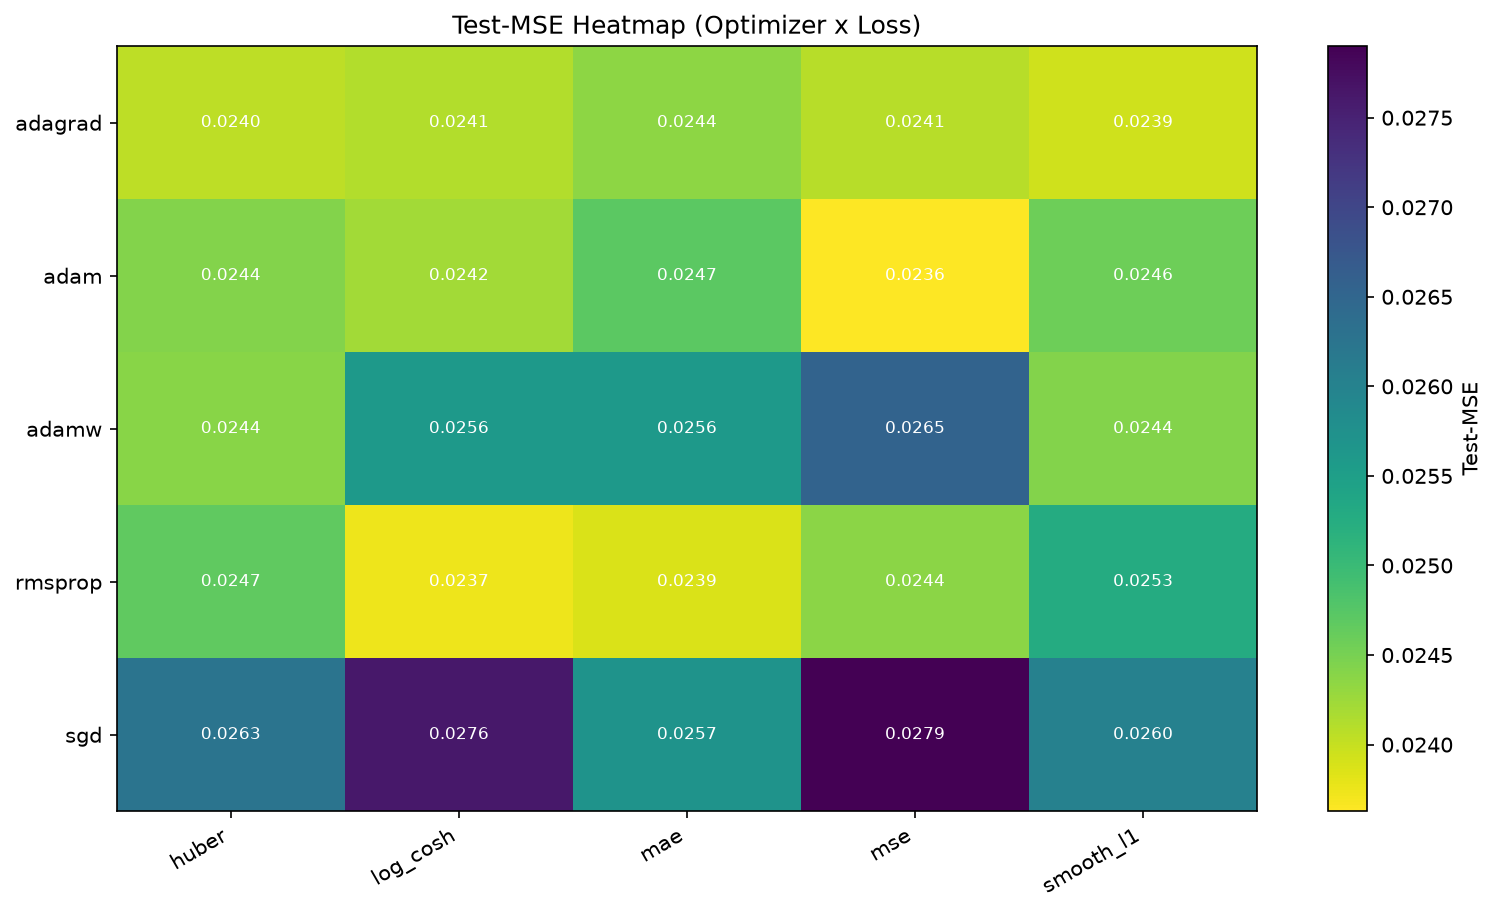
\includegraphics[width=\textwidth]{heatmap_test_mse.png}
    \caption{Heatmap der Test-\gls{MSE}-Werte für die systematische Grid-Search-Evaluation unterschiedlicher Loss-Funktionen und Optimizer-Strategien auf Basis der unregularisierten 2-Layer-\gls{GRU}-Architektur.}
    \label{fig:loss_optimizer_heatmap}
\end{figure}

Die zeilenweise Auswertung der Optimierungsalgorithmen offenbart ein noch prägnanteres Leistungsgefälle. Das klassische Stochastische Gradientenabstieg-Verfahren (\gls{SGD}) versagt in diesem Setup unabhängig von der gewählten Loss-Funktion komplett und weist die signifikant schlechteste Generalisierung auf (dunkelviolette Zeile mit Werten von bis zu 0.0279 beim \gls{MSE}). 
Adaptive Algorithmen dominieren das Feld sichtbar und stabilisieren das Training auf einem durchgehend höheren Niveau. 
\gls{Adagrad} besticht dabei durch eine enorme Konstanz über alle Fehlerfunktionen hinweg und erzielt den besten mittleren Test-\gls{MSE} der Optimizer-Familien (0.0241). 
\gls{RMSprop} zeigt mit \gls{MAE} und Log-Cosh (jeweils unter 0.0240) ebenfalls extrem starke Resultate. 
Dennoch erreicht die \gls{Adam}-Variante in der Spitze das absolute globale Optimum.

Basierend auf dieser direkten Auswertung der Heatmap wird das finale \gls{BC}-Modell mit dem \gls{Adam}-Optimizer und dem \gls{MSE}-Loss kompiliert. 
Diese Konfiguration stellt empirisch belegt die maximale Vorhersagegüte für die nun tiefer dimensionierte Netzwerkstruktur sicher.



    \newpage

    \section{Implementierung und Training}

\subsection{Entwicklungsumgebung}
Dieses Kapitel dokumentiert die verwendete Hardware, Software und Frameworks (Python, PyTorch) zur Sicherstellung der wissenschaftlichen Reproduzierbarkeit.

\subsection{Implementierung der Data Pipeline}

\subsubsection{Dataset-Klassen}
Dieser Abschnitt beschreibt die Programmierung der PyTorch-Schnittstelle zum Einlesen und Vorhalten der bereinigten Betriebsdaten.

\subsubsection{DataLoader und Batch-Generierung}
Es werden Laderoutinen zur iterativen Übergabe der Zeitreihenpakete (Batches) an das Modell umgesetzt.

\subsection{Trainingsschleife und Hyperparameter-Tuning}
Die programmierte Trainingsschleife wird dokumentiert, einschließlich Festlegung und Begründung von Learning Rates, Batch-Sizes und Early-Stopping-Kriterien.

    \newpage

    \section{Evaluierung und Ergebnisse}

\subsection{Evaluierungsmetriken und Test-Setup}
Dieses Kapitel definiert die quantitativen Error-Metriken (MSE, MAE) zur Leistungsmessung und etabliert den Bewertungsmaßstab auf dem isolierten Test-Set.

\subsection{Ergebnisse des Behavior Cloning}

\subsubsection{Quantitative Loss-Analyse}
Es erfolgt die Auswertung und Interpretation der berechneten Metriken sowie der Train- vs. Validation-Loss-Kurven zum Nachweis verhinderter Überanpassung.

\subsubsection{Visuelle Verhaltensanalyse}
Dieser Abschnitt stellt die vorhergesagten Actions (Hebelstellungen) und die Ground Truth (Fahrereingaben) grafisch über die Zeit gegenüber.

\subsection{Vergleichende RL-Evaluierung (Warm Start vs. Cold Start)}
Es werden die Reward-Kurven eines Agenten mit und ohne Pre-Training in der Simulation gegenübergestellt und der zeitliche sowie qualitative Performance-Gewinn quantifiziert.

\subsection{Diskussion und Limitationen}
Dieses Kapitel interpretiert die erzielten Ergebnisse objektiv und ordnet verbleibende Fehlerquellen (Covariate Shift) sowie Limitationen im Datensatz kritisch ein.

    \newpage

    \section{Fazit und Ausblick}

\subsection{Zusammenfassung}

Ausgangspunkt der vorliegenden Arbeit war die Beobachtung, dass Reinforcement-Learning (RL)-Agenten im Schienenverkehr ohne eine geeignete Initialisierung kaum konvergieren und bei einer rein simulativen Offline-Initialisierung zudem das Risiko des Overfittings auf spezifische Trainingsstrecken besteht. Als Reaktion darauf verfolgte diese Arbeit das Ziel, mittels Behavior Cloning (BC) ein neuronales Netz zu entwickeln, das reale Fahrstrategien menschlicher Triebfahrzeugführer aus historischen Betriebsdaten erlernt und damit als robuste, generalisierbare Baseline für einen zukünftigen Warm-Start von RL-Agenten dienen kann.

Zur Erreichung dieser Zielsetzung wurde ein iteratives, experimentelles Vorgehen gewählt. Nach einer theoretischen Fundierung zu Supervised Learning, BC und geeigneten Netzwerkarchitekturen folgte eine ausführliche Exploratory Data Analysis der realen Betriebsdaten, auf deren Grundlage eine deterministische Preprocessing- und Feature-Engineering-Pipeline entwickelt wurde. Über ein fahrtenbasiertes Trip-Level-Splitting wurde sichergestellt, dass Trainings-, Validierungs- und Testmenge vollständig disjunkte, unabhängige Fahrten enthalten und Data Leakage auf Zeitschrittebene ausgeschlossen ist. In einem dreistufigen Auswahlprozess wurden anschließend Architektur, Netzwerkgröße sowie Optimierer und Verlustfunktion empirisch bestimmt; als finale Konfiguration ergab sich ein LSTM mit der Layer-Konfiguration 128-64-256-128 (650.369 Parameter), trainiert mit Adam und Smooth-L1-Loss. Über fünf Trainingsiterationen wurden Rauschen und Gewichtsinitialisierung, Batch-Size sowie zyklische Regularisierungstechniken systematisch angepasst, bevor das finale Modell auf dem vollständigen Trainingsdatensatz trainiert wurde.

Die abschließende Evaluation auf der bis dahin unangetasteten Testmenge zeichnet ein gemischtes Bild: Auf den unmittelbar über den quadratischen Fehler definierten Metriken ($R^2$, RMSE, MSE) übertrifft das Modell eine strenge Persistenz-Baseline deutlich, während es bei MAE sowie bei Richtungs- und Toleranz-Accuracy hinter dieser zurückbleibt. Die klassenweise Analyse identifiziert die Ursache: Seltene, aber sicherheitsrelevante Bremsanforderungen werden mit einem Recall von lediglich 3,2\,\% nahezu systematisch verpasst, während das Modell in den weitaus häufigeren, ruhigen Beharrungsphasen präzise Vorhersagen liefert. Dieses Verhalten lässt sich plausibel auf die begrenzte Datenbasis von 1.388 Trips bzw. rund 178 Stunden Aufzeichnungszeit zurückführen, in der Extremmanöver naturgemäß unterrepräsentiert sind. Insgesamt liefert das entwickelte Modell damit keine im vollen Umfang optimalen, aber für den angestrebten Machbarkeitsnachweis hinreichende Ergebnisse.

\subsection{Beantwortung der Forschungsfrage}
\label{subsec:forschungsfrage}

Um die eingangs formulierte Forschungsfrage fundiert beantworten zu können, wird zunächst auf die Erreichung der drei in Abschnitt~\ref{subsec:zielsetzung} definierten Teilziele eingegangen, bevor eine zusammenfassende Bewertung der Forschungsfrage selbst erfolgt.

Das erste Teilziel, die Transformation der unstrukturierten Rohdaten in eine strukturierte, für das maschinelle Lernen nutzbare Repräsentation, wurde vollständig erreicht. Mittels der in Kapitel~\ref{sec:daten_preprocessing} entwickelten EDA- und Feature-Engineering-Pipeline konnten zentrale, fahrphysikalisch kausale Input-Features wie Streckengradient, Geschwindigkeit und Distanz zu Stoppstellen identifiziert und in einen wohldefinierten Zustands- sowie Aktionsraum überführt werden. Die dabei entstandene deterministische Pipeline stellt zugleich sicher, dass Preprocessing und Feature-Auswahl für alle nachfolgenden Experimentierschritte reproduzierbar bleiben.

Auch das zweite Teilziel, die Konzeptionierung und Implementierung einer geeigneten Deep-Learning-Architektur, wurde erreicht. Der in Kapitel~\ref{sec:konzeption} durchgeführte dreistufige Auswahlprozess führte zu einer LSTM-Architektur, die in der Lage ist, die nicht-linearen, zeitlich abhängigen Zusammenhänge zwischen den topologischen Streckendaten und der kontinuierlichen Zielgröße abzubilden. Sowohl die Netzwerkdimensionierung als auch die Wahl von Optimierer und Verlustfunktion wurden dabei empirisch abgesichert und nicht willkürlich festgelegt.

Das dritte Teilziel, die Verhinderung von Overfitting bei gleichzeitiger Sicherstellung der Generalisierungsfähigkeit, wurde nur teilweise erreicht. Durch das fahrtenbasierte Trip-Level-Splitting sowie die in Kapitel~\ref{sec:training} angewandten Regularisierungstechniken generalisiert das Modell nachweislich auf vollständig ungesehene Fahrten und übertrifft die Persistenz-Baseline bei den regressionsbasierten Metriken. Gleichzeitig zeigt die in Kapitel~\ref{sec:evaluation} durchgeführte klassenweise Analyse, dass diese Generalisierung nicht gleichmäßig über alle Fahrsituationen hinweg gelingt: Insbesondere für seltene, dynamische Brems- und Beschleunigungsmanöver bleibt die Generalisierungsfähigkeit deutlich hinter der für ruhige Beharrungsphasen erreichten Güte zurück.

Auf dieser Grundlage lässt sich die zentrale Forschungsfrage, ob sich aus unstrukturierten historischen Betriebsdaten ein künstliches neuronales Netz trainieren lässt, das eine generalisierbare Fahrstrategie für Züge erlernt, mit einem begründeten Ja beantworten. Der im Rahmen dieser Arbeit erbrachte Machbarkeitsnachweis zeigt, dass ein solches Training grundsätzlich möglich ist: Das Modell erlernt aus realen, unstrukturierten Sensordaten eine Policy, die auf ungesehenen Testfahrten insgesamt bessere Regressionsergebnisse liefert als eine triviale Fortschreibungsstrategie und in ruhigen Fahrsituationen sehr präzise Vorhersagen trifft. Zugleich macht die Arbeit jedoch deutlich, dass die Qualität einer solchen Policy unmittelbar von der zur Verfügung stehenden Datenmenge abhängt: Gerade die für eine sichere und vollständig generalisierbare Fahrstrategie entscheidenden, aber seltenen Extremmanöver konnten aufgrund der vergleichsweise kleinen Datenbasis von 178 Stunden nicht robust erlernt werden. Dies ist zugleich der zentrale Grund dafür, dass die erzielten Ergebnisse am Ende dieser Arbeit nicht als optimal, wohl aber als für den angestrebten Machbarkeitsnachweis ausreichend zu bewerten sind. Die Forschungsfrage ist damit im Grundsatz positiv, aber mit der wesentlichen Einschränkung einer ausreichend großen und hinsichtlich seltener Ereignisse hinreichend reichhaltigen Datenbasis zu beantworten.

\subsection{Kritische Reflexion}

Trotz des grundsätzlich positiven Machbarkeitsnachweises sind mehrere Aspekte des gewählten Vorgehens kritisch zu hinterfragen.

Zunächst betrifft dies die Zusammensetzung der Datenbasis selbst. Da sämtliche Trips von einer einzigen, homogenen Güterverkehrsstrecke stammen, konnte kein streckenübergreifendes Splitting vorgenommen werden; die in Abschnitt~\ref{subsec:finale_testevaluation} beschriebene Dominanz von Rangier- und Anfahrsituationen im Testset ist eine unmittelbare Folge dieser Datengrundlage. Die berichteten Metriken sind somit zunächst nur für diese spezifische Strecke und das zugrundeliegende Fahrzeug- bzw. Führerprofil aussagekräftig; inwieweit die erlernte Policy auf andere Streckentypen, Zuggattungen oder Traktionsarten übertragbar ist, kann im Rahmen dieser Arbeit nicht beurteilt werden.

Methodisch ist zudem die ausgeprägte Klassenimbalance zwischen Halte-, Brems- und Beschleunigungsanforderungen zu nennen. Die verwendete Smooth-L1-Verlustfunktion optimiert den Gesamtfehler primär über die zahlenmäßig dominierenden, unauffälligen Zeitschritte, wodurch seltene, aber sicherheitsrelevante Ereignisse systematisch unterrepräsentiert bleiben. Gezielte Gegenmaßnahmen wie eine klassengewichtete Verlustfunktion oder ein gezieltes Oversampling dynamischer Fahrabschnitte wurden in dieser Arbeit bewusst nicht eingesetzt, um die Vergleichbarkeit der in Kapitel~\ref{sec:konzeption} und~\ref{sec:training} durchgeführten Experimente nicht zusätzlich zu verkomplizieren; ihr Fehlen dürfte jedoch zu der beobachteten, unzureichenden Erkennung von Bremsanforderungen beigetragen haben.

Auch der gewählte methodische Rahmen des Behavior Cloning selbst ist limitiert: Da das Modell rein offline auf historischen Zustands-Aktions-Paaren trainiert wurde, ohne jemals mit den Konsequenzen eigener Entscheidungen in einer geschlossenen Regelschleife konfrontiert zu sein, bleibt unklar, wie sich kleine, im Training unvermeidbare Abweichungen von der menschlichen Referenz im tatsächlichen Einsatz akkumulieren würden. Die in Abschnitt~\ref{sec:problemstellung} beschriebene Gefahr des Extrapolationsfehlers bei ungesehenen Situationen wurde durch das Trip-Level-Splitting zwar für die Evaluation, nicht aber für einen realen, sequenziellen Einsatz methodisch adressiert.

Schließlich wurden die Trainings-Hyperparameter Lernrate, Batch-Size, Weight Decay und Dropout-Rate während der Architektur- und Dimensionierungsexperimente in Kapitel~\ref{sec:konzeption} bewusst auf feste Startwerte gesetzt, um die Vergleichbarkeit der jeweils untersuchten Designentscheidung sicherzustellen. Dies erhöht zwar die interne Validität der einzelnen Experimentstufen, schließt jedoch nicht aus, dass eine gemeinsame, gekoppelte Optimierung von Architektur und Hyperparametern zu einer anderen finalen Konfiguration und potenziell besseren Ergebnissen geführt hätte.

\subsection{Ausblick}

Ausgehend von der in Abschnitt~\ref{subsec:kritische_einordnung} sowie Abschnitt~\ref{subsec:forschungsfrage} identifizierten Kernursache der beobachteten Schwächen ergibt sich als naheliegendste Anschlussarbeit die Erweiterung der zugrunde liegenden Datenbasis. Da sich die Modellgüte gerade bei seltenen Brems- und Beschleunigungsmanövern unmittelbar an der geringen Anzahl entsprechender Trainingsbeispiele festmachen lässt, würde bereits eine Verdopplung oder Verdreifachung der aufgezeichneten Betriebsstunden die absolute Zahl solcher Extremereignisse proportional erhöhen und damit voraussichtlich zu einer spürbar robusteren Erkennung dynamischer Fahrsituationen führen. Ergänzend dazu erscheinen datengetriebene Maßnahmen wie eine klassengewichtete Verlustfunktion oder ein gezieltes Oversampling unterrepräsentierter Manöver als vielversprechende, vergleichsweise aufwandsarme nächste Schritte.

Der zentrale nächste Schritt liegt jedoch, wie bereits in der Zielsetzung dieser Arbeit angelegt, in der eigentlichen Nutzung des entwickelten Modells als Warm-Start-Initialisierung für einen Reinforcement-Learning-Agenten. Anstatt einen RL-Agenten wie in Abschnitt~\ref{sec:problemstellung} beschrieben ohne fachliche Vorprägung und mit dem damit verbundenen Risiko einer mangelnden Konvergenz zu initialisieren, kann die in dieser Arbeit trainierte BC-Policy als Startpunkt dienen, von dem aus im Anschluss ein RL-Training durchgeführt wird. Auf diesem Weg ließe sich untersuchen, ob und in welchem Umfang sich das Fahrverhalten des Agenten durch anschließendes Reinforcement Learning gegenüber der reinen BC-Baseline tatsächlich verbessern lässt – insbesondere in genau jenen dynamischen Übergangsphasen, in denen das in dieser Arbeit entwickelte Modell noch die größten Schwächen zeigt. Erst eine solche kombinierte Warm-Start-plus-RL-Strategie würde damit das übergeordnete, in Abschnitt~\ref{subsec:zielsetzung} formulierte Ziel dieser Arbeit vollständig einlösen: eine zuverlässige, generalisierbare Fahrstrategie für den automatisierten Schienenverkehr bereitzustellen.
    \newpage

    % Literaturverzeichnis
    \sloppy % Lockert die Anforderungen an die Zeilenlänge
    \raggedright
    \printbibliography[title=Literaturverzeichnis,heading=bibnumbered]
    \newpage
    % Anhang
    \appendix
    \section{Nutzung von Künstlicher Intelligenz}
    \label{sec:anhang-ki}

    \begin{table}[htbp]
        \centering
        \refstepcounter{table}
        \label{tab:ki-nutzung}
        \vspace{0.5em}
        \begin{tabular}{>{\raggedright\arraybackslash}p{0.28\textwidth} p{0.62\textwidth}}
            \toprule
            \textbf{Hilfsmittel} & \textbf{Verwendung} \\
            \midrule
            Gemini Pro 3.1 & Planung und Strukturierung der Arbeitsweise \\
            Gemini Flash 3.7 & Schnelle Fragenbeantwortung und Verständnisfragen \\
            Claude Sonnet 5 & Hilfe bei Formulierungen \\
            Claude Opus 4.8 in GitHub Copilot & Codegenerierung sowie Hilfe beim Debugging und Code-Fixing \\
            \bottomrule
        \end{tabular}
    \end{table}

\end{document}